% ============================================================================
% 第 6 章  Fukaya 范畴  （原书 pp.85–109，PDF pp.88–112）
% ============================================================================
\section{Fukaya 范畴}\label{ch:06}

% 原书公式在全书范围内连续编号：本章自 (78) 起、至 (100) 止，共 23 个编号公式。
% main.tex 已采用全局连续编号；此处补设计数器为 77，保证本章首个编号公式
% 恰为 (78)。若前几章的公式计数已经连续到 77，则本行只是空操作。
\setcounter{equation}{77}

\takeaway{%
  核心图像：Fukaya 范畴以拉格朗日子流形为对象、以 Floer 复形为态射空间，
  合成映射 $\mu^d$ 由伪全纯多边形的带权计数给出；对象间的“几何运算”
  （映射锥）具体化为 Dehn 扭转与拉格朗日连通和。\\
  数学工具：伪全纯圆盘与条带的模空间、Maslov 指标、结合面体 $K_d$、
  非幺 $A_\infty$-范畴、扭复形与 Yoneda 嵌入。\\
  主要结论：$\mu^d$ 满足 $A_\infty$-结合关系（命题 6.12），上同调范畴与
  三角包络分别是 Donaldson–Fukaya 范畴与 $\mathsf D^\pi(\mathcal F(M))$；
  沿球面的 Dehn 扭转与沿单点横截相交的连通和都等于映射锥
  （定理 6.23、定理 6.28）；wrapped 版本以卷绕哈密顿量处理非紧正合流形。%
}

\subsection{Floer 乘积}\label{sec:6.1}

我们引入第三条拉格朗日子流形，并改造上一章的几何构造，以便在两个 Floer
复形之间定义一个乘积，即 \emph{Floer 乘积}。主要参考文献是 \cite{Aur13}
第 2 节。

照例考虑近复辛流形 $M^{2n}=(M,\omega,J)$，其中 $2c_1(TM)=0$ 且
$J\in\mathcal J(M,\omega)$；再取三条拉格朗日子流形 $L_0,L_1,L_2\subset M$，
假定它们紧致、可定向、自旋、分次，Maslov 类消没，且不包围任何冒泡。
此外设它们两两横截相交：$L_i\pitchfork L_j$ 对 $i\neq j\in\{0,1,2\}$ 成立。
此时横截性、紧致性与可定向性都容易实现（一般情形稍后讨论）。我们要找的
是相应 Floer 复形之间如下形式的乘积运算：
\[
CF(L_1,L_2)\otimes CF(L_0,L_1)\longrightarrow CF(L_0,L_2)\,.
\]

参照图~\ref{fig:05}，研究如下问题：给定 $p_1\in\mathcal X(L_0,L_1)$、
$p_2\in\mathcal X(L_1,L_2)$、$q\in\mathcal X(L_0,L_2)$（此处暂时
$\mathcal X(L_i,L_j)=L_i\cap L_j$），以及点
$z_1=e^{-i\pi/3}$、$z_2=e^{i\pi/3}$、$z_0=-1\in S^1$，我们要找
$J$-全纯映射 $u:\mathbb D^2\setminus\{z_0,z_1,z_2\}\to M$ 满足边界条件
\begin{equation}
\left\{
\begin{aligned}
&u(e^{i\alpha})\in L_0 \quad \text{若}\ \alpha\in\bigl(-\pi,-\tfrac{\pi}{3}\bigr)
&&\text{且}\ \lim_{z\to z_0}u(z)=q\,,\\[2pt]
&u(e^{i\alpha})\in L_1 \quad \text{若}\ \alpha\in\bigl(-\tfrac{\pi}{3},\tfrac{\pi}{3}\bigr)
&&\text{且}\ \lim_{z\to z_1}u(z)=p_1\,,\\[2pt]
&u(e^{i\alpha})\in L_2 \quad \text{若}\ \alpha\in\bigl(\tfrac{\pi}{3},\pi\bigr)
&&\text{且}\ \lim_{z\to z_2}u(z)=p_2\,,
\end{aligned}
\right.
\label{eq:6.78}
\end{equation}
并且能量有限，$E(u)<\infty$。它们是某个适当表述的 Cauchy--Riemann 问题的解
（见下文式 \eqref{eq:6.81}），由此得到的同伦类
$[u]\in\pi_2(M,L_0\cup L_1\cup L_2)$ 定义了模空间
$\mathcal M(p_1,p_2,q;[u],J)$；得益于关于紧致性与横截性的假设，后者是有限维
光滑流形。与 Floer 微分一样，所求的乘积运算要对所有这些 $J$-全纯映射作带权
计数；如图~\ref{fig:05} 所示，它们也可称为 \emph{伪全纯三角形}。

\begin{figure}[htbp]
  \centering
  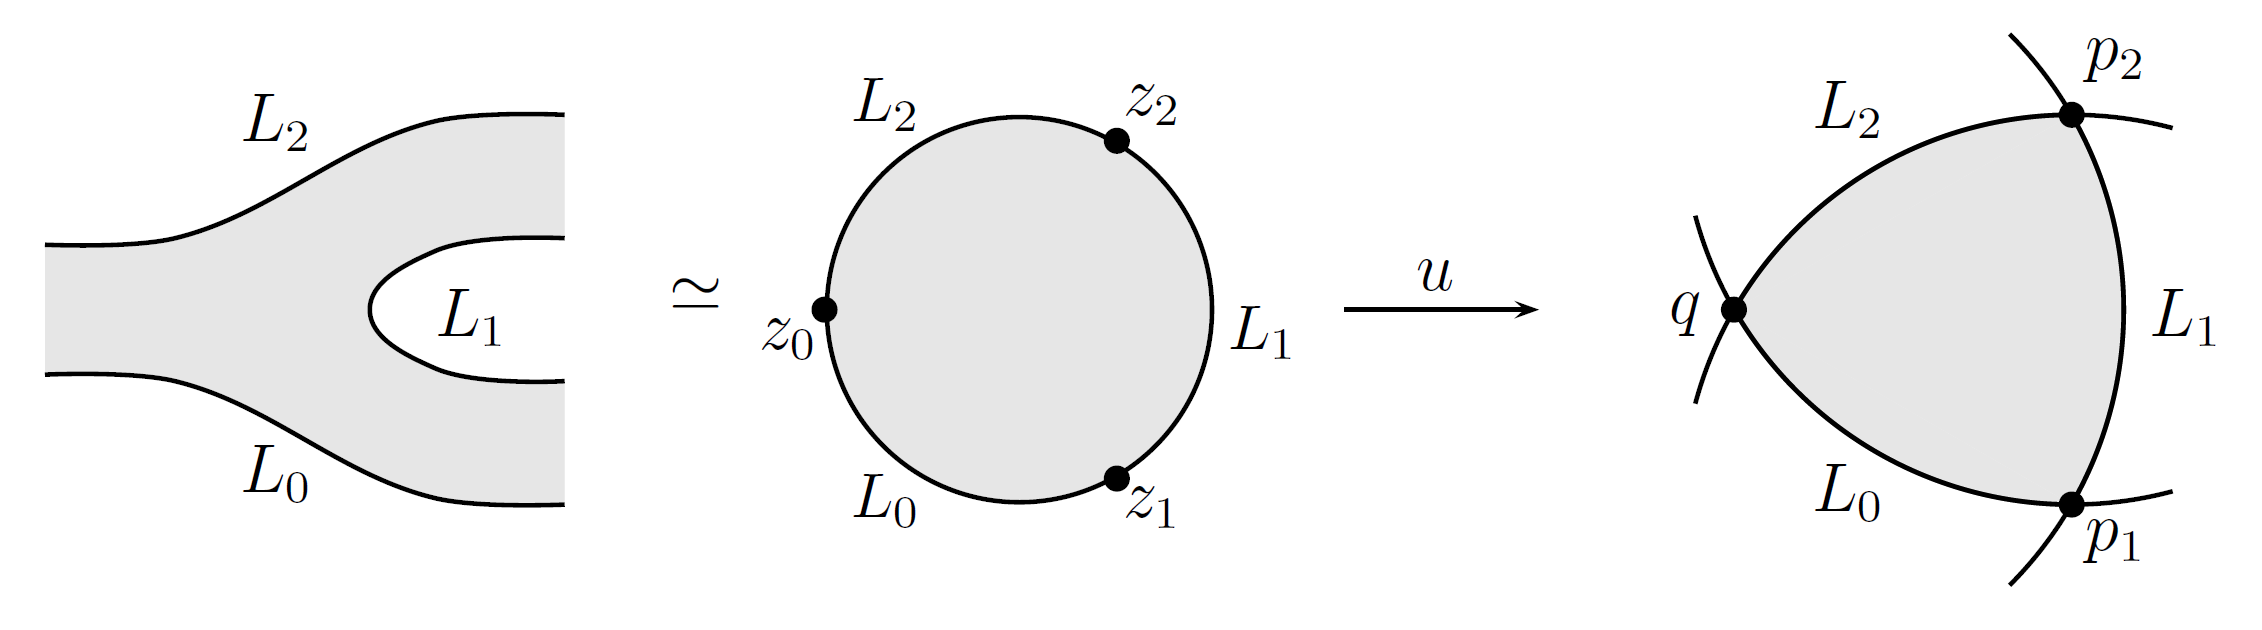
\includegraphics[width=0.9\linewidth]{fig05.png}
  \caption{属于 $\mathcal M(p_1,p_2,q;[u],J)$ 的一条三穿孔 $J$-全纯圆盘 $u$。\hfill（原书 p.85）}
  \label{fig:05}
\end{figure}

\begin{Rem}\label{rem:6.1}
与 (57)--(59) 的相似之处显而易见。事实上，$\mathbb D^2$ 中每个“穿孔” $z_i$
的充分小开邻域都双全纯于 $\mathbb R\times[0,1]\subset\mathbb R^2\cong\mathbb C$，
图~\ref{fig:05} 正强调了这一点：它给出了三穿孔圆盘
$\mathbb D^2\setminus\{z_0,z_1,z_2\}$ 与左端“三端条带”之间的一个双全纯映射。

另一方面，图 2 已经暗示了 $\mathbb D^2\setminus\{\pm1\}$ 与
$\mathbb R\times[0,1]$ 的等同。因此人们可以——而且马上会看到，也应当——
把问题 \eqref{eq:6.78} 理解为第 5 章所讨论内容的“$3$ 次类比”。
\end{Rem}

% [Tutor Note: 【易错】式 (78) 的三段边界弧以 $z_0=-1$、$z_1=e^{-i\pi/3}$、
% $z_2=e^{i\pi/3}$ 为分界点：与 $\mathbb R\times[0,1]$ 的端点 $\pm1$ 不同，
% 这里三段弧的长度都是 $2\pi/3$。计数时三个穿孔点的循环次序固定在
% $\operatorname{Aut}(\mathbb D^2)$ 轨道下才不依赖 $z_j$ 的具体位置。]

注意，与定义 5.12 不同，我们并不要求用 $\mathbb R$ 去除
$\mathcal M(p_1,p_2,q;[u],J)$，因为解空间上不存在整体的自由平移作用。
事实上，自同构群 $\operatorname{Aut}(\mathbb D^2)$ 在带标记边界点的循环有序
三元组上传递作用，所以连 $z_j$ 的选取也无关紧要。于是
$\mathcal M(p_1,p_2,q;[u],J)$ 的维数直接等于 Maslov 指标
$\operatorname{ind}([u])$：

\begin{Lem}\label{lem:6.2}
设 $M^{2n}=(M,\omega,J)$ 是近复辛流形，$2c_1(TM)=0$，而
$L_0,L_1,L_2\subset M$ 是如上拉格朗日子流形，特别地分次且
$[\phi_{L_i}]=0$。则成立
\[
\dim\bigl(\mathcal M(p_1,p_2,q;[u],J)\bigr)
=\operatorname{ind}([u])=\deg(q)-\deg(p_1)-\deg(p_2)\,.
\]
（同样，这也等于由 $D_{\bar\partial_{J,u}}$ 定义的 Fredholm 指标。）
\end{Lem}

\begin{proof}[证明（概要）]
只需改造第 5.4 节给出的 Maslov 指标定义。暂记 $q:=p_0$，沿
$\partial(\operatorname{im}(u))$ 逆时针行进：先把 $u^*TM$ 适当平凡化，
再考虑定义 5.17 所述从 $T_{p_j}L_j$ 到 $T_{p_k}L_j$ 的道路 $l_i$，以及从
$T_{p_i}L_k$ 到 $T_{p_i}L_i$ 的典范短道路 $\lambda_{p_i}$，其中
$(i,j,k)$ 遍取 $(0,1,2)$ 的循环置换；然后研究以 $T_{p_0}L_0$ 为基点的环路
\[
\gamma_u:=l_2*\lambda_{p_1}*l_0*\lambda_{p_2}*l_1*\lambda_{p_0}
\in LGr(n)\,.
\]
定义 5.22 关于生成元次数的论述在此仍成立（并且由我们的假设而有意义）。
于是所断言的等式来自道路拼接下的可加性。
\end{proof}

% [Tutor Note: 【易错】引理 6.2 的指标位移是关键：输出端点 $q$ 贡献
% $+\deg(q)$，两个输入端点各贡献一个负号。这正是 $\mu^2$ 度数为
% $0=2-2$、$\mu^d$ 度数为 $2-d$ 的来源（式 (83)、(84)）。]

% [Tutor Note: 【背景】证明中的环路 $\gamma_u$ 按
% $l_2,\lambda_{p_1},l_0,\lambda_{p_2},l_1,\lambda_{p_0}$ 交错拼接；
% 若把 $(i,j,k)$ 的循环置换写错方向，会得到反向环路，Maslov 指标相差一个
% 符号。原文按逆时针参数化，与第 5 章定义 5.17 的约定一致。]

引理 6.2 的证明还表明，$CF(L_1,L_2)\otimes CF(L_0,L_1)$ 带有由两个 Floer
复形自然诱导的 $\mathbb Z$-分次（特别地
$\deg(p_2\otimes p_1)=\deg(p_2)+\deg(p_1)$）。

\begin{Def}\label{def:6.3}
设 $M=(M,\omega,J)$ 是近复辛流形，$2c_1(TM)=0$，而
$L_0,L_1,L_2\subset M$ 是带通常装饰的拉格朗日子流形，特别地满足
$\langle\omega\rangle\cdot\pi_2(M,L_i)=0$。\emph{Floer 乘积}
$\cdot:CF(L_1,L_2)\otimes CF(L_0,L_1)\to CF(L_0,L_2)$ 是下述映射的
$\Lambda_{\mathbb K}$-线性延拓：
\begin{equation}
p_2\otimes p_1\longmapsto p_2\cdot p_1
:=\sum_{\substack{q\in\mathcal X(L_0,L_2)\\ [u]:\ \operatorname{ind}([u])=0}}
\bigl(\#\mathcal M(p_1,p_2,q;[u],J)\bigr)\,T^{\omega([u])}\,q\,,
\label{eq:6.79}
\end{equation}
其中 $\mathcal M(p_1,p_2,q;[u],J)$ 是 Cauchy--Riemann 问题 \eqref{eq:6.78}
代表 $[u]\in\pi_2(M,L_0\cup L_1\cup L_2)$ 的解构成的模空间。式
\eqref{eq:6.79} 中的求和良定义（论证同定理 5.39 的证明），而引理 6.2
告诉我们 $\cdot$ 是 $0$ 次映射。
\end{Def}

% [Tutor Note: 【易错】式 (79) 的下标条件写作“[u]: ind([u])=0”，
% 它不是对生成元 $q$ 求和时的附加条件，而是对同伦类求和的范围；
% 对一般的 $(p_1,p_2,q)$ 只有有限多个类满足此条件（由能量下界与
% $\langle\omega\rangle\cdot\pi_2(M,L_i)=0$ 保证）。]

下面考察 Floer 乘积相对于 Floer 微分的核心性质：它满足分次 Leibniz 法则。
我们借助其背后的几何论证来微调微扰、时间依赖近复结构与哈密顿量的选取。

\begin{Pro}\label{pro:6.4}
Floer 乘积满足分次 Leibniz 法则
\begin{equation}
\partial(p_2\cdot p_1)=(-1)^{|p_1|}\partial(p_2)\cdot p_1
-p_2\cdot\partial(p_1)\,,
\label{eq:6.80}
\end{equation}
其中 $|p_1|:=\deg(p_1)$，且各 $\partial$ 是定义 5.37 给出的适当 Floer 微分。
因此，上同调上诱导的乘积
$HF(L_1,L_2)\otimes HF(L_0,L_1)\to HF(L_0,L_2)$ 良定义，并且实际上与
所涉及的微扰数据的选取无关（参见其证明）。
\end{Pro}

% [Tutor Note: 【易错】式 (80) 的符号 $(-1)^{|p_1|}$ 只加在
% $\partial(p_2)\cdot p_1$ 一项上；这是 Koszul 符号法则在“微分是
% 分次导子”上的体现。若把 $p_1,p_2$ 的次序或符号放反，会与
% 式 (85) 中 $d=2$ 的 $A_\infty$-关系差一个整体符号。]

\begin{proof}[证明（概要）]
我们定性解释其中的几何想法，并对照定理 5.39 证明中的做法。取图~\ref{fig:05} 中那样的
生成元 $p_1\in\mathcal X(L_0,L_1)$、$p_2\in\mathcal X(L_1,L_2)$、
$q\in\mathcal X(L_0,L_2)$，以及同伦类
$[u]\in\pi_2(M,L_0\cup L_1\cup L_2)$，设 $\operatorname{ind}([u])=1$。
假定横截性成立，则 $\mathcal M(p_1,p_2,q;[u],J)$ 是光滑 $1$ 维流形；由
Gromov 紧致性定理 5.34，它可以紧化为某个
$\overline{\mathcal M}(p_1,p_2,q;[u],J)$，只需补上断裂条带（按假设，
圆盘冒泡与球面冒泡均被排除）。

但现在有三个“条带状”端点可以聚集能量。由 Maslov 指标在条带断裂下的可加性、
圆盘的指标非负（横截性使然），以及非常值条带的指标至少为 $1$，指标分解
$\operatorname{ind}([u])=\operatorname{ind}([u'])+\operatorname{ind}([u''])$
只有三种可能：适当重新命名后，$u'$ 必是某条指标 $1$ 的条带，而 $u''$ 是以
$L_0,L_1,L_2$ 为边界的指标 $0$ 圆盘。\footnote{这与我们按假设排除的圆盘冒泡
不同：后者的边界落在单条子流形上，并且是唯一能导致能量爆破的圆盘。}
说白了，我们只需把伪全纯三角形 $u$ 在一个角上“捏紧”，见图~\ref{fig:06}。具体地说，
图中所示三种构型分别贡献 $\partial(p_2\cdot p_1)$、$p_2\cdot\partial(p_1)$
与 $\partial(p_2)\cdot p_1$ 中 $T^{\omega([u])}q$ 的系数。

\begin{figure}[htbp]
  \centering
  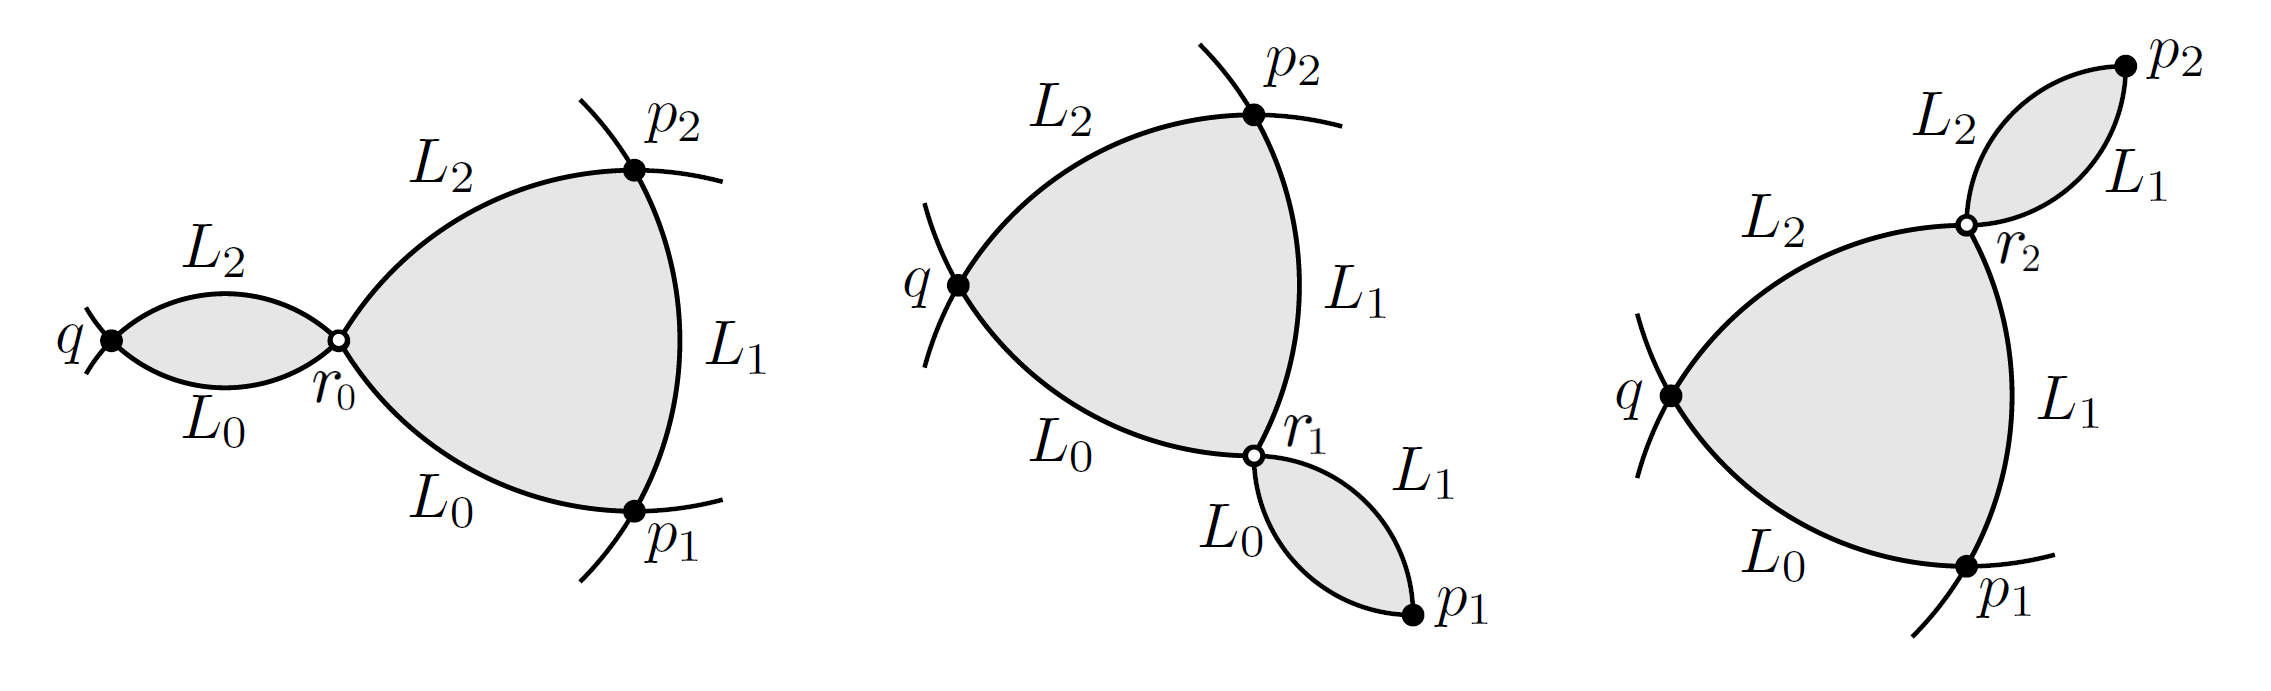
\includegraphics[width=0.9\linewidth]{fig06.png}
  \caption{$\mathcal M(p_1,p_2,q;[u],J)$ 中三穿孔 $J$-全纯圆盘的三类可能极限构型。\hfill（原书 p.87）}
  \label{fig:06}
\end{figure}

这意味着 $\partial\overline{\mathcal M}(p_1,p_2,q;[u],J)$ 包含在形如
$\mathcal M(p_i,r_i;[u'],J)\times\mathcal M(r_i,p_j,p_k;[u''],J)$ 的模空间
乘积的无交并之中，其中 $r_j\in\mathcal X(L_i,L_j)$ 是“捏紧”得到的点
（仍记 $q:=p_0$）。反向包含由另一个粘接定理给出，于是
$\overline{\mathcal M}(p_1,p_2,q;[u],J)$ 确实是紧致 $1$ 维光滑流形，
其边界如上所述（且定向相容）。引理 5.38 告诉我们，后者的（带符号或无符号）
基数为零；对所有同伦类求和并仔细计及次数，即得 Leibniz 法则
\eqref{eq:6.80}。

至于式 \eqref{eq:6.79} 在上同调上诱导出良定义乘积，论证十分容易：若
$\partial(p_1)=\partial(p_2)=0$，则由 \eqref{eq:6.80} 得
$\partial(p_2\cdot p_1)=0$；若再有 $p_1=\partial(p_1')$，则
$p_2\cdot p_1=\partial(p_2\cdot p_1')$。因此闭上链与上边界都被保持，正是
所愿。
\end{proof}

% [Tutor Note: 【含糊】证明中“反向包含由另一个粘接定理给出”省略了
% 全部分析细节：需要先在每条指标 1 的条带与指标 0 的三角形之间建立
% 预粘接（pre-glue），再证明粘接映射是微分同胚。完整论证见
% \cite{Sei08} 第 9 章与 \cite{FOOO09} 第 7–8 章；本译本不补写。]

最后讨论 $L_i\not\pitchfork L_j$ 的一般情形。为达到横截性，我们重新引入
时间依赖的近复结构与哈密顿量：对每个条带状端点取一对
$(J_{ij},H_{ij})\in C^\infty([0,1],\mathcal J(M,\omega))\times
C^\infty([0,1]\times M)$，按所界定的拉格朗日子流形标记
$0\le i<j\le 2$（见图~\ref{fig:05} 左）。注意由注 6.1，这样做是合理的。然而
这一次，这样的数据无法延拓到整个穿孔圆盘：必须选取整体定义的
$J\in C^\infty(\mathbb D^2,\mathcal J(M,\omega))$ 与
$H\in C^\infty(\mathbb D^2\times M)$（即随 $\mathbb D^2$ 光滑变化的族），
使它们在每个 $z_j$ 的固定邻域内与所选的 $(J_{ij},H_{ij})$ 相符。

于是我们只在穿孔附近恢复微扰方程 (66)，那里可以使用全纯局部复坐标
$z=s+it$，$(s,t)\in\mathbb R\times[0,1]$。为看清这一点，取
$\beta\in\Omega^1(\mathbb D^2)$ 使 $\beta|_{S^1}=0$ 且在诸 $z_j$ 附近
$\beta=dt$。微扰 Cauchy--Riemann 方程 (57)，得到
\begin{equation}
(du-X_H\otimes\beta)^{0,1}_J=0\,,
\label{eq:6.81}
\end{equation}
它在三个穿孔附近恰与 Floer 方程重合：
$0=(du-X_H\otimes dt)^{0,1}_J=\partial_s u+J_t(u)(\partial_t u-X_{H_t}(u))$，
其中 $J$ 与 $H$ 仅依赖 $t$。与第 5.5 节所得类似，有
$\mathcal X(L_i,L_j)=L_i\cap(\phi^1_{H_{ij}})^{-1}(L_j)$；上面几段的证明
可原样搬到微扰乘积映射
$\cdot:CF(L_1,L_2;J_{12},H_{12})\otimes CF(L_0,L_1;J_{01},H_{01})
\to CF(L_0,L_2;J_{02},H_{02})$ 上，于是它满足 Leibniz 法则。

% [Tutor Note: 【易错】式 (81) 中 $\beta$ 在 $S^1$ 上为零、在穿孔附近为 $dt$，
% 因此 $(du-X_H\otimes\beta)^{0,1}_J$ 的微扰项只在穿孔附近出现；若取
% $\beta=dt$ 整体定义，则方程不再与 Floer 方程局部相符。另注意
% $(\,\cdot\,)^{0,1}_J$ 是 $J$-反线性部分的投影，$\beta$ 是实 $1$-形式。]

\subsection{高阶复合映射}\label{sec:6.2}

现在考虑涉及 $(d+1)$ 条拉格朗日子流形 $L_0,\dots,L_d\subset M$ 的高阶乘积，
它们带有通常的装饰。

给定 $d+1$ 个生成元 $p_1\in\mathcal X(L_0,L_1)$，
$p_2\in\mathcal X(L_1,L_2)$，……，
$p_d\in\mathcal X(L_{d-1},L_d)$，$q\in\mathcal X(L_d,L_0)$，以及边界穿孔
$z_j=e^{i\pi(1+2j/(d+1))}$、$z_0=-1\in S^1$（$j=1,\dots,d$）；我们要找
$J$-全纯映射 $u:\mathbb D^2\setminus\{z_0,z_1,\dots,z_d\}\to M$，满足微扰
Cauchy--Riemann 方程 \eqref{eq:6.81} 的 $(d+1)$ 次类比，边界条件为
\begin{equation}
\left\{
\begin{aligned}
&u(e^{i\alpha})\in L_0 \quad \text{若}\ \alpha\in\Bigl(\pi,\pi+\tfrac{2\pi}{d+1}\Bigr)
&&\text{且}\ \lim_{z\to z_0}u(z)=q\,,\\[2pt]
&u(e^{i\alpha})\in L_j \quad \text{若}\ \alpha\in\Bigl(\pi+\tfrac{2j\pi}{d+1},\pi+\tfrac{2(j+1)\pi}{d+1}\Bigr)
&&\text{且}\ \lim_{z\to z_j}u(z)=p_j\,,
\end{aligned}
\right.
\label{eq:6.82}
\end{equation}
并且能量有限，$E(u)<\infty$。我们称其为\emph{广义 Cauchy--Riemann 问题}。
代表固定同伦类 $[u]\in\pi_2\bigl(M,\bigcup_{i=0}^d L_i\bigr)$ 的解构成模空间
$\mathcal M(p_1,\dots,p_d,q;[u],J,H)$。情形如图~\ref{fig:07} 所示，该图也说明为何
$J$-全纯解 $u$ 的像 $\operatorname{im}(u)$（进而 $u$ 本身）被称为
\emph{伪全纯多边形}。

这里我们已经选取了适当的、依赖定义域的
$J\in C^\infty(\mathbb D^2,\mathcal J(M,\omega))$ 与
$H\in C^\infty(\mathbb D^2\times M)$，并注意（见下文定义 6.9）如下事实：
与上一节 $d=2$ 的情形不同，此处循环有序元组
$(z_0,z_1,\dots,z_d)\subset S^1$ 有许多选法，区别在于每个穿孔在其弧上的
确切相对位置。

\begin{Def}\label{def:6.5}
设 $\operatorname{Punct}_{d+1}$ 是边界穿孔的一切有序构型
$(z_0,z_1,\dots,z_d)\subset S^1$ 构成的空间（$d\ge 2$），
$\operatorname{Aut}(\mathbb D^2)$ 是 $\mathbb D^2$ 的双全纯群。则
$\mathcal M_{0,d+1}:=\operatorname{Punct}_{d+1}/\operatorname{Aut}(\mathbb D^2)$
是 $\mathbb D^2$ 上\emph{共形结构}的模空间，它是一个可缩的 $(d-2)$ 维
光滑流形。
\end{Def}

\begin{figure}[htbp]
  \centering
  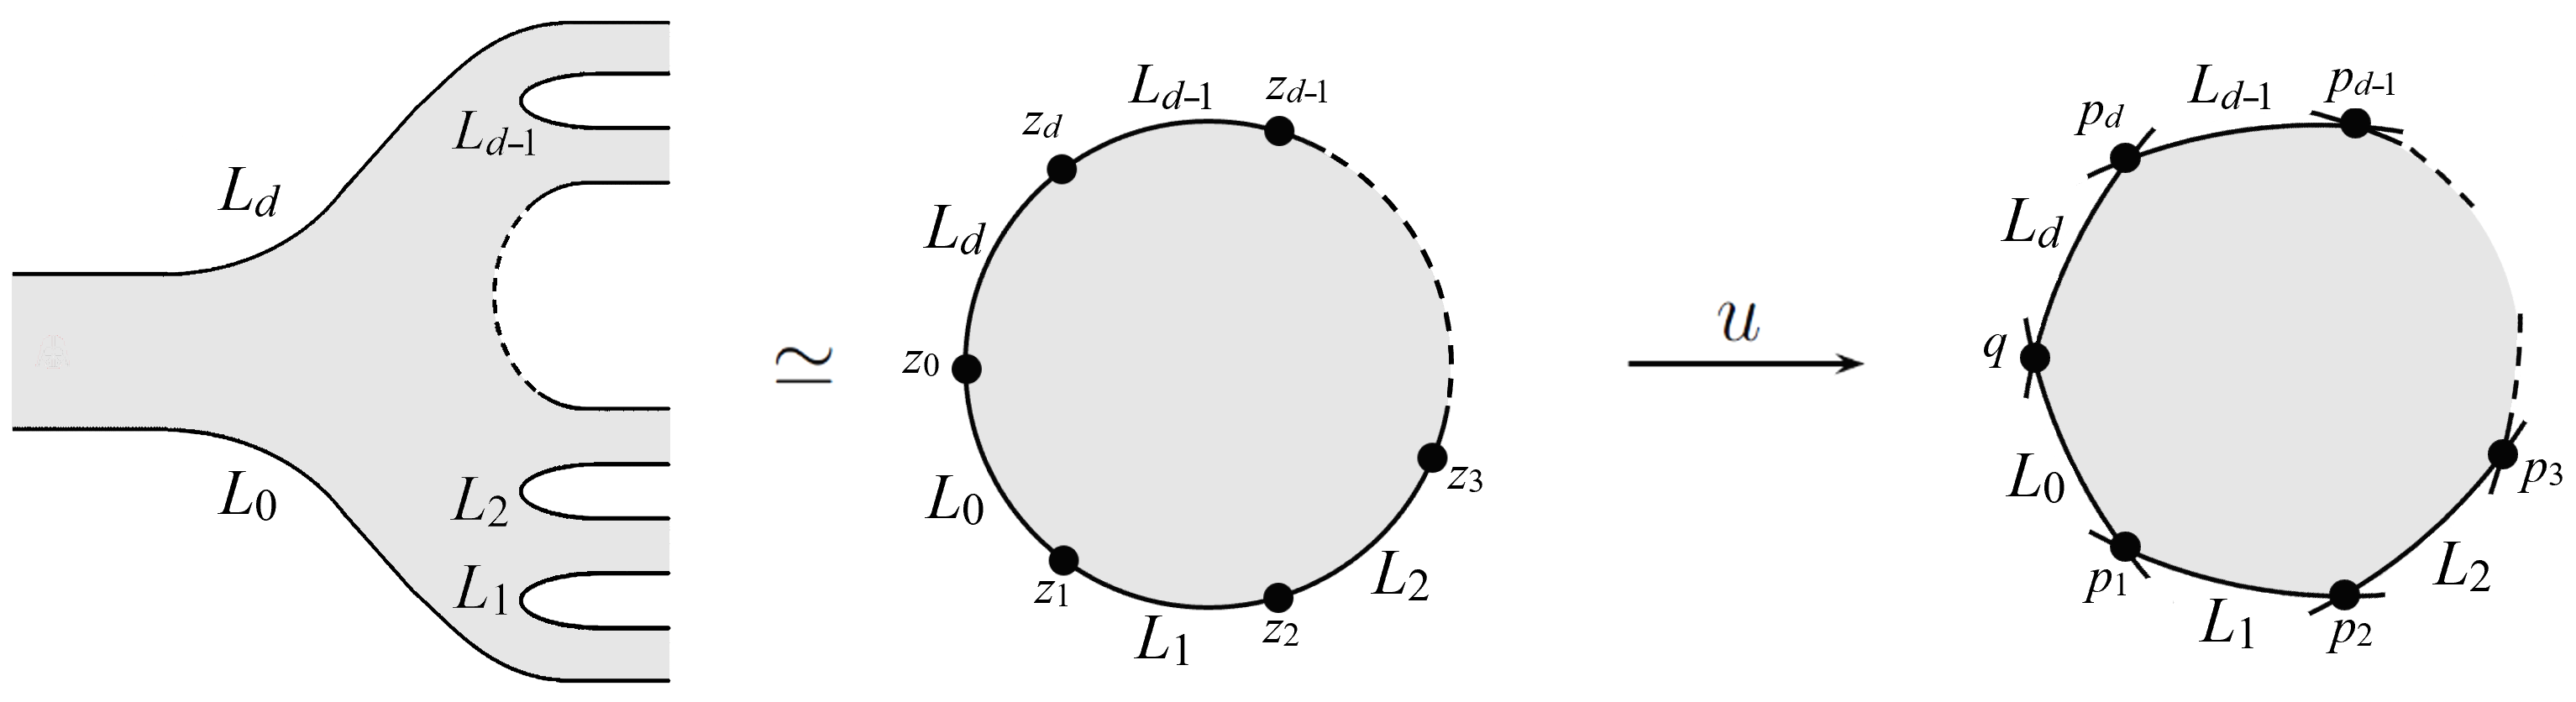
\includegraphics[width=0.9\linewidth]{fig07.png}
  \caption{属于 $\mathcal M(p_1,\dots,p_d,q;[u],J,H)$ 的一条 $(d+1)$-穿孔 $J$-全纯圆盘 $u$。\hfill（原书 p.89）}
  \label{fig:07}
\end{figure}

空间 $\mathcal M_{0,d+1}$ 有自然的紧化，得到 $(d-2)$ 维多胞形
$\overline{\mathcal M}_{0,d+1}$——（同胚地）正是我们在第 1.1 节遇到的
结合面体 $K_d$！其边界 $\partial\overline{\mathcal M}_{0,d+1}$ 参数化
$\mathbb D^2$ 的一切可能退化（\emph{节点退化}），退化为若干子圆盘，每个
至少携带一个穿孔 $z_j$。具体地说，每个 $(d-3)$-骨架分支对应一类（同伦类
意义下的）退化为两个圆盘、每个至少保留两个穿孔；同样，$(d-4)$-骨架可
指派三个圆盘的构型，如此类推。

% [Tutor Note: 【背景】$\mathcal M_{0,d+1}$ 的维数是 $d-2$：$d+1$ 个边界
% 穿孔在 $S^1$ 上共 $d+1$ 个自由度，商去 $\operatorname{Aut}(\mathbb D^2)$
% 的 $3$ 个自由度，得 $d-2$。紧化把它添成结合面体 $K_d$，其面的偏序
% 恰对应括号的插入方式；这正是 $A_\infty$-关系的几何来源。]

\begin{Ex}\label{ex:6.6}
设 $d=3$。我们知道紧化的 $1$ 维多胞形 $\overline{\mathcal M}_{0,4}=K_3$
同胚于 $[0,1]\subset\mathbb R$（见图 1 左下）。构成其 $0$-骨架的两个端点
标记 $\mathbb D^2$ 在固定穿孔 $z_1,z_2,z_3\in S^1$ 时（不失一般性）的两种
可能退化：或者 $z_0\in S^1$ 可沿 $L_0$ 向 $z_1$ “滑动”，最终与它一起落入
对应 $0$ 的退化构型的某个子圆盘中；或者它沿 $L_3$ 向 $z_3$ 滑动，产生
对应 $1$ 的构型（见图~\ref{fig:08}）。
\end{Ex}

\begin{figure}[htbp]
  \centering
  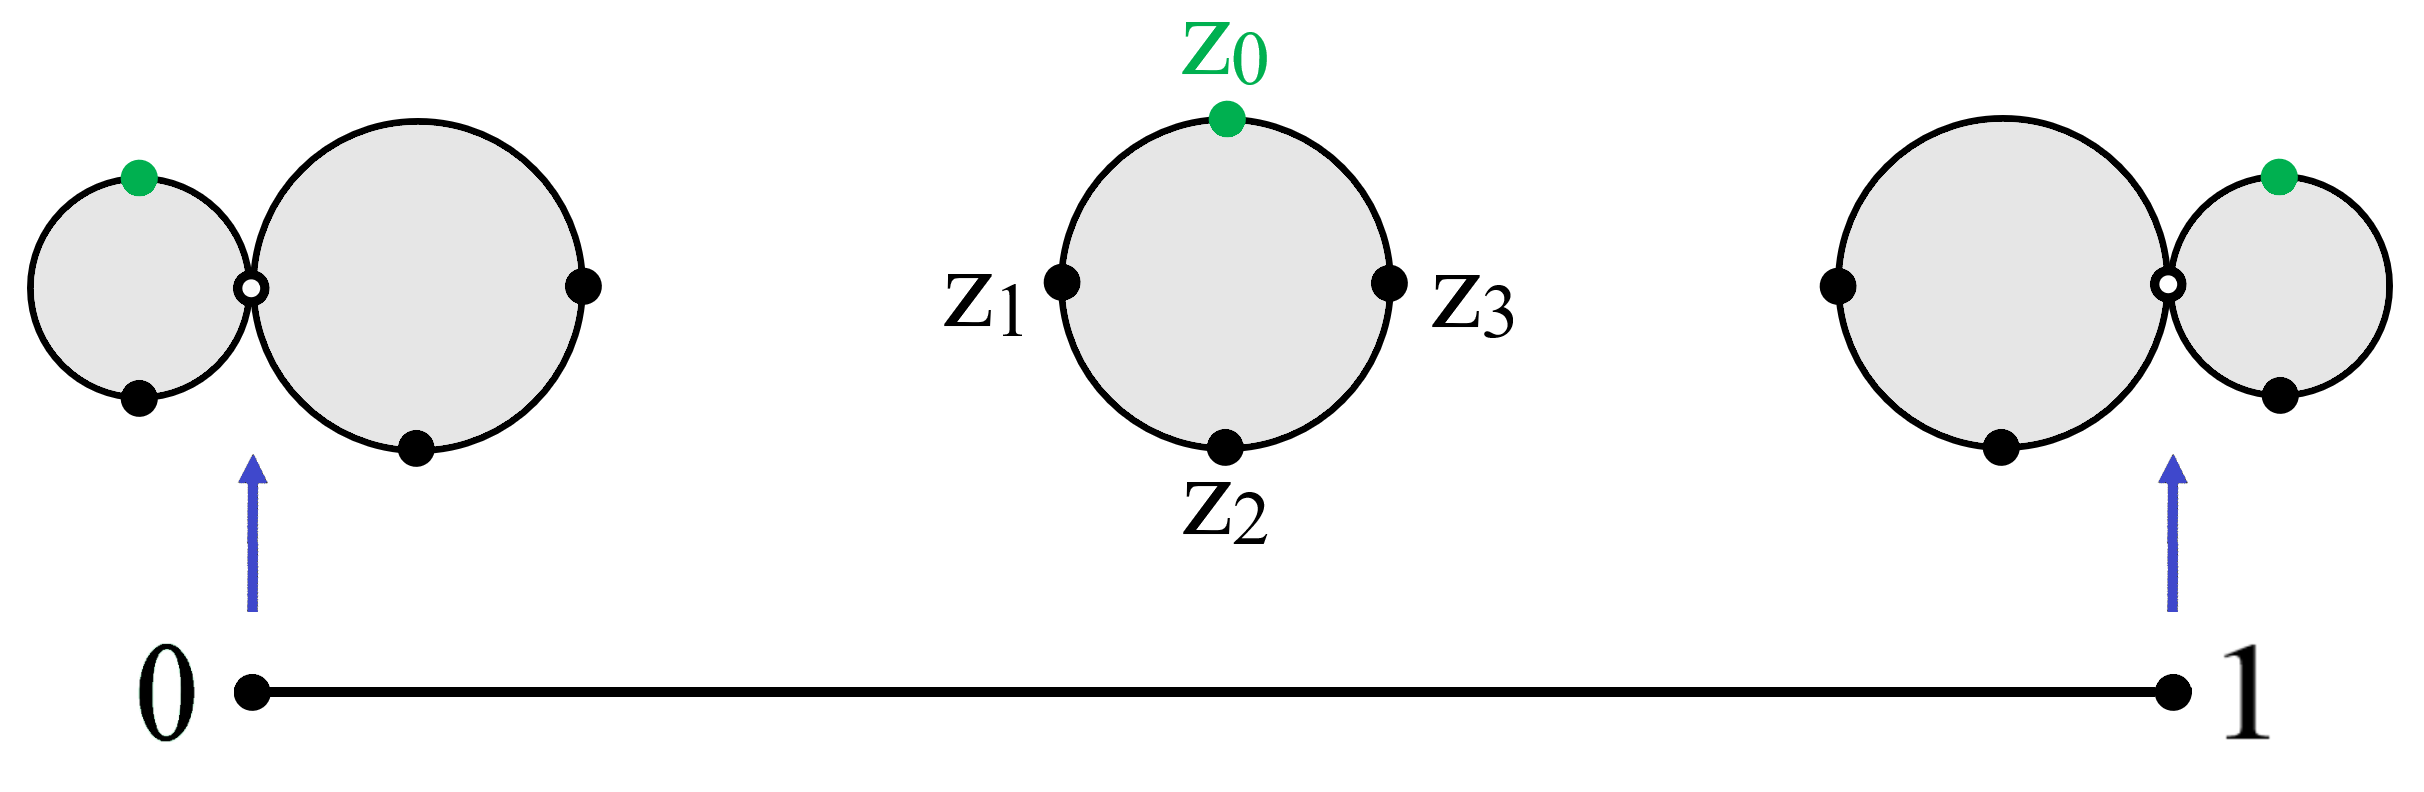
\includegraphics[width=0.8\linewidth]{fig08.png}
  \caption{多胞体 $\overline{\mathcal M}_{0,4}=K_3$ 及其对应的退化极限构型（白点表示新生成的节点）。\hfill（原书 p.89）}
  \label{fig:08}
\end{figure}

换个方式，我们也可固定 $z_0,z_1,z_2$ 而让 $z_3$ 变动。这个“滑动操作”
——由第 1.1 节的同伦 $m_3$ 形式化——会对 Floer 复形上的某些高阶复合映射
作出贡献，下面将予以说明。

\begin{Rem}\label{rem:6.7}
在上一个例子的基础上，可以如下解释 $\mathcal M_{0,d+1}$ 的定义。群
$\operatorname{Aut}(\mathbb D^2)\cong PSL(2,\mathbb R)$ 是 $3$ 维 Lie 群，
其作用至多能唯一固定 $\mathbb D^2$ 的三个边界穿孔（事实上
$\mathcal M_{0,3}=\operatorname{Punct}_3/\operatorname{Aut}(\mathbb D^2)$
是 $0$ 维的，故可忽略，正如紧接注 6.1 之后的讨论所示）。若 $d>2$，
即若处理多于三个穿孔，则这些穿孔可自由地沿映入拉格朗日子流形的弧滑动，
从而在 $\mathcal M_{0,d+1}$ 中产生非平凡的不同类。模去可被固定的三个穿孔，
便知 $\mathcal M_{0,d+1}$ 具有 $(d+1)-3=d-2$ 维光滑流形的结构。

与例 6.6 类似，当两个或更多穿孔撞在一起时，$\mathbb D^2$ 便发生节点退化，
由此产生冒泡效应；该效应消解为若干携带相关点的子圆盘。$\mathcal M_{0,d+1}$
的紧化就是把这类极限构型一并纳入，它们由 $\partial\overline{\mathcal M}_{0,d+1}$
标定。
\end{Rem}

\begin{Ex}\label{ex:6.8}
对 $\overline{\mathcal M}_{0,5}=K_4$ 的直观理解如下。给定五个穿孔
$z_0,z_1,z_2,z_3,z_4\in S^1$，固定一个（相邻的！）三元组，比如
$z_1,z_2,z_3$，而让 $z_0,z_4$ 变动。我们有十种方式让这一对“相撞”。
例如 $z_0$ 可以撞上 $z_1$，我们不妨将其写作 $(z_0*z_1)$。其余组合为
（沿图~\ref{fig:09} 逆时针移动）：
$(z_4*(z_0*z_1))$、$(z_4*z_0*z_1)$、$((z_4*z_0)*z_1)$、
$(z_4*z_0)$、$(z_3*(z_4*z_0))$、$(z_3*z_4*z_0)$、
$((z_3*z_4)*z_0)$、$(z_3*z_4)$ 以及 $(z_0*z_1)(z_3*z_4)$。

括号至关重要，因为它们规定了碰撞的次序！事实上，$(z_4*z_0*z_1)$ 对应
退化为两个子圆盘、其中一个携带 $z_0,z_1,z_4$ 的节点退化；而
$(z_4*(z_0*z_1))$ 编码三个圆盘的构型，其中间的圆盘携带 $z_4$，末端的
圆盘收集 $z_0$ 与 $z_1$。显然，所列组合中有五个标定五边形 $K_4$ 的边
（即其 $1$-骨架），另外五个标定其顶点（$0$-骨架）。
\end{Ex}

\begin{figure}[htbp]
  \centering
  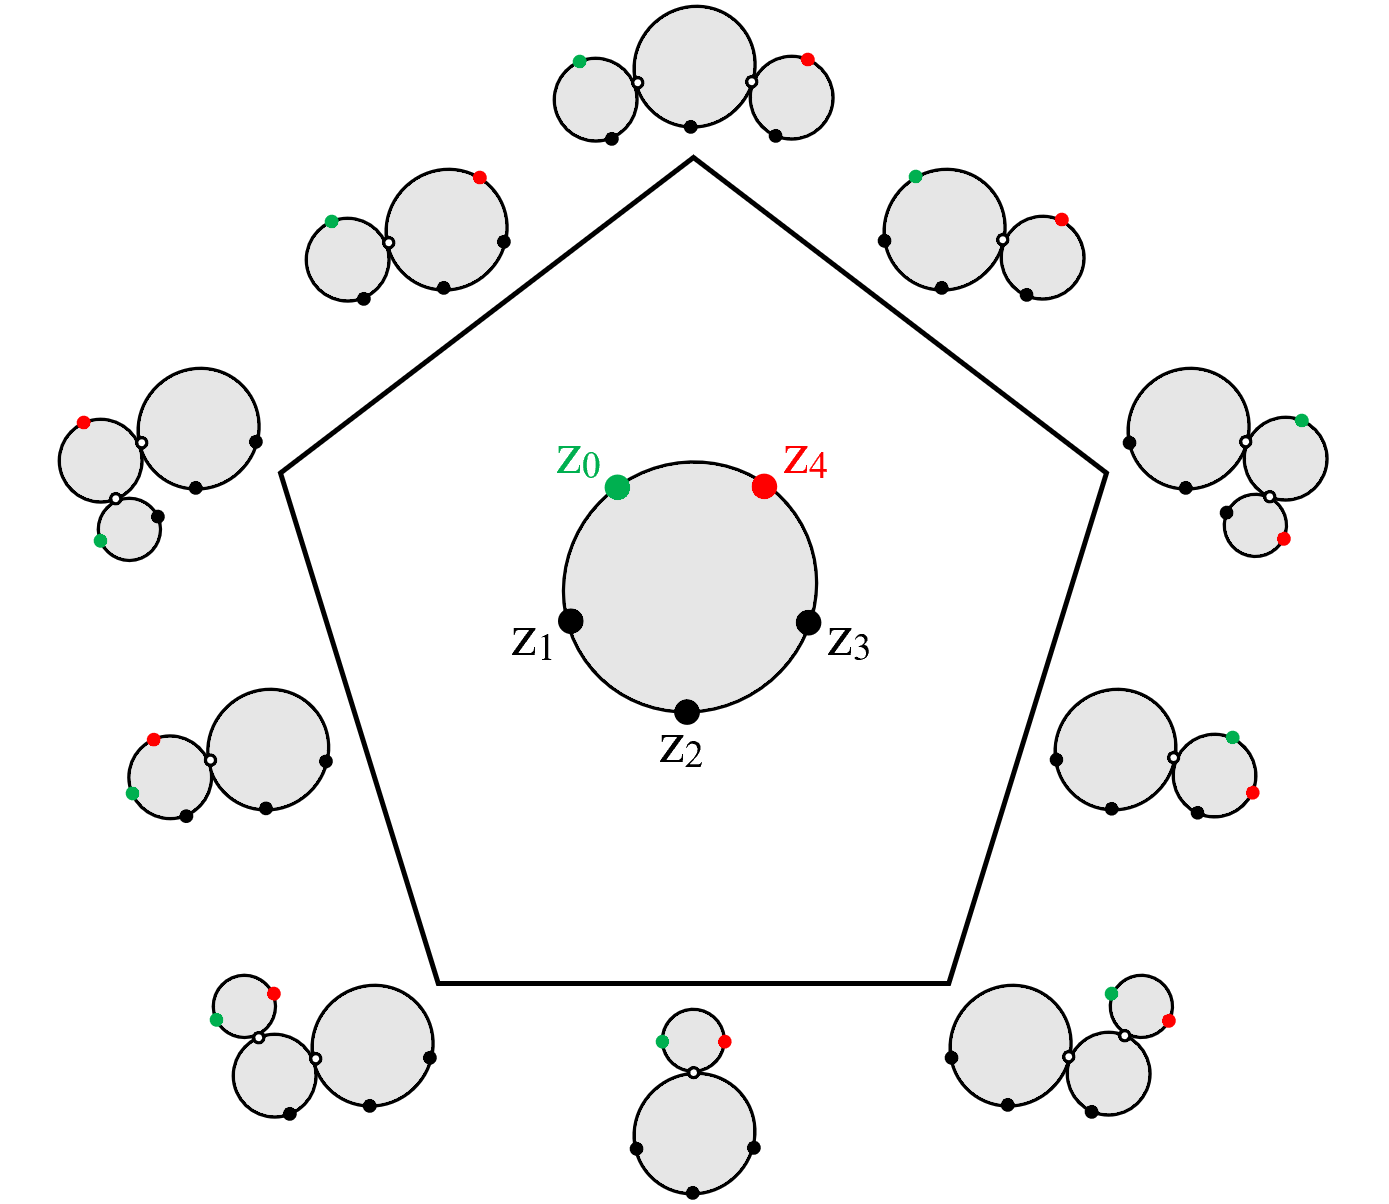
\includegraphics[width=0.55\linewidth]{fig09.png}
  \caption{多胞体 $\overline{\mathcal M}_{0,5}=K_4$ 及其对应的退化极限构型（白点表示新生成的节点）。\hfill（原书 p.90）}
  \label{fig:09}
\end{figure}

我们有意让变量保持循环次序，以凸显另一种解释：$K_d$ 的
$(d-r)$-骨架分支对应于在字符串 $z_0z_1\cdots z_{d-1}z_d$ 中适当插入
$r-2$ 对括号。例如
$(z_4*(z_0*z_1))\equiv(z_0z_1))z_2z_3(z_4$。这使得研究高维结合面体大大
简化。读者不妨考察 $K_5$（图 1 中最右侧者），其九个面、二十一条边与
十四个顶点分别参数化退化为两个、三个与四个子圆盘的可能节点退化。

% [Tutor Note: 【勘误】“$(z_4*(z_0*z_1))\equiv(z_0z_1))z_2z_3(z_4$”这一
% 括号串在原书中括号不平衡（左括号与右括号数目不等）。原文如此印，
% 疑为“$(z_0z_1))z_2z_3(z_4$”想表达的是把 $z_4$ 与 $(z_0*z_1)$ 分别
% 归入两个子圆盘的括号插入；译文照印，读者理解其意即可，勿据此做符号推导。]

最后说明在 $d+1$ 条拉格朗日子流形的一般情形下如何选取相容的微扰数据。
其存在性的证明见 \cite{Sei08} 引理 9.5。

\begin{Def}\label{def:6.9}
给定共形结构 $(z_0,z_1,\dots,z_d)\in\mathcal M_{0,d+1}$，考虑相应的、
形如 \eqref{eq:6.81}、带边界条件 \eqref{eq:6.82} 与有限能量约束的广义
Cauchy--Riemann 问题。再考虑确定 $CF(L_i,L_j)$ 的时间依赖
$(J_{ij},H_{ij})\in C^\infty([0,1],\mathcal J(M,\omega))\times
C^\infty([0,1]\times M)$，对每个条带状端点（即定义在 $p_j$ 与 $q$ 的固定
邻域上、可用全纯局部坐标之处）按所界定的拉格朗日子流形标记
$0\le i<j\le d$。为达到横截性，我们选取
$J\in C^\infty(\mathbb D^2,\mathcal J(M,\omega))$ 与
$H\in C^\infty(\mathbb D^2\times M)$，使得：
\begin{itemize}
  \item $(J,H)$ 在相应的条带状端点上与每个 $(J_{ij},H_{ij})$ 相符；
  \item 按定义 6.5 的方式使 $\mathbb D^2$ 节点退化时，$J$ 与 $H$ 在节点
  周围的（条带状）区域中平移不变，并且确实与那里的局部哈密顿量及近复结构
  重合。
\end{itemize}
我们称这样的对 $(J,H)$ 为 \emph{Floer 数据}；由构造，它依赖于
$(z_0,z_1,\dots,z_d)$ 以及所有 $J_{ij}$ 与 $H_{ij}$。于是由此产生的 Floer
上同调称为“无障碍的（unobstructed）”。
\end{Def}

% [Tutor Note: 【含糊】“Floer 数据”的相容性只是逐条列出的要求，原文并未
% 构造它；存在性完全依赖 \cite{Sei08} 引理 9.5 的归纳构造（逐次在
% 结合面体的骨架上延拓）。所谓“unobstructed”指 $\mu^0=0$、从而
% $A_\infty$-关系不被圆盘冒泡破坏，而非指模空间自动正则。]

$\mathcal M_{0,d+1}$ 的介入还意味着必须相应改造引理 6.2 及其证明。

\begin{Lem}\label{lem:6.10}
固定共形结构 $(z_0,z_1,\dots,z_d)\in\mathcal M_{0,d+1}$ 及如上述相容的
Floer 数据 $(J,H)\in C^\infty(\mathbb D^2,\mathcal J(M,\omega))\times
C^\infty(\mathbb D^2\times M)$。考虑相应的广义 Cauchy--Riemann 问题，它对
每个解 $[u]\in\pi_2\bigl(M,\bigcup_{i=0}^d L_i\bigr)$ 给出模空间
$\mathcal M(p_1,\dots,p_d,q;[u],J,H)$。则
\begin{equation}
\begin{aligned}
\dim\bigl(\mathcal M(p_1,\dots,p_d,q;[u],J,H)\bigr)
&=\dim(\mathcal M_{0,d+1})+\operatorname{ind}([u])\\
&=d-2+\deg(q)-\sum_{i=1}^{d}\deg(p_i)\,,
\end{aligned}
\label{eq:6.83}
\end{equation}
其中 $\dim(\mathcal M_{0,d+1})$ 计入 $(z_0,z_1,\dots,z_d)$ 的可能形变。
\end{Lem}

\begin{Def}\label{def:6.11}
设 $(M,\omega,J)$ 是近复辛流形，$2c_1(TM)=0$，而 $L_0,\dots,L_d\subset M$
是带通常装饰的拉格朗日子流形，特别地满足
$\langle\omega\rangle\cdot\pi_2(M,L_i)=0$。选取 Floer 数据
$(J,H)\in C^\infty(\mathbb D^2,\mathcal J(M,\omega))\times
C^\infty(\mathbb D^2\times M)$ 以达到横截性。第 $d$ 个 \emph{Floer 复合映射}
$\mu^d:CF(L_{d-1},L_d)\otimes\cdots\otimes CF(L_0,L_1)\to CF(L_0,L_d)$
是下述映射的 $\Lambda_{\mathbb K}$-线性延拓：
\begin{equation}
\mu^d(p_d,\dots,p_1):=\sum_{\substack{q\in\mathcal X(L_0,L_d)\\
[u]:\ \operatorname{ind}([u])=2-d}}
\bigl(\#\mathcal M(p_1,\dots,p_d,q;[u],J,H)\bigr)\,
T^{\omega([u])}\,q\,,
\label{eq:6.84}
\end{equation}
\end{Def}

其中 $\mathcal M(p_1,\dots,p_d,q;[u],J,H)$ 是广义 Cauchy--Riemann 问题
\eqref{eq:6.81} 代表 $[u]\in\pi_2\bigl(M,\bigcup_{i=0}^d L_i\bigr)$ 的解
构成的模空间。按通常论证，该求和良定义；并且注意引理 6.10 使 $\mu^d$
成为次数 $2-d$ 的分次映射。

特别地，$\mu^1=\partial_{J,H}$ 是（$1$ 次的）Floer 微分 (74)，而
$\mu^2=\cdot$ 是（$0$ 次的）Floer 乘积 \eqref{eq:6.79}。

% [Tutor Note: 【易错】式 (84) 的指标条件 $\operatorname{ind}([u])=2-d$
% 必须与式 (83) 联读：由 $\dim(\mathcal M)=d-2+\operatorname{ind}([u])$
% 及 $\operatorname{ind}([u])=2-d$ 知所计数的模空间是 $0$ 维的；而式 (83)
% 的另一个表达式给出 $\deg(q)-\sum_i\deg(p_i)=2-d$。换言之，指标条件
% $\operatorname{ind}=2-d$ 正是“$\mu^d$ 的度数为 $2-d$”的另一种说法。
% 这也是 $\mu^1$ 为 $1$ 次、$\mu^2$ 为 $0$ 次的原因。]

\begin{Pro}\label{pro:6.12}
Floer 复合映射 $\mu^d$ 满足 $A_\infty$-结合关系 (6)：
\begin{equation}
\sum_{\substack{1\le m\le d\\ 0\le n\le d-m}}(-1)^{\dagger_n}\,
\mu^{d-m+1}\bigl(p_d,\dots,p_{n+m+1},
\mu^m(p_{n+m},\dots,p_{n+1}),p_n,\dots,p_1\bigr)=0\,,
\label{eq:6.85}
\end{equation}
在 $CF(L_0,L_d)$ 中成立，其中 $p_i\in CF(L_{i-1},L_i)$，且
$\dagger_n:=\bigl(\sum_{i=1}^{n}|p_i|\bigr)-n$。\footnote{鉴于式
\eqref{eq:6.85}，我们的确用 $|p_i|$ 取代了 $\deg(p_i)$。}
\end{Pro}

对 $d=1,2$，前两个这样的方程即 $\partial(\partial(p_1))=0$ 与
$\partial(p_2\cdot p_1)=(-1)^{|p_1|}\partial(p_2)\cdot p_1
-p_2\cdot\partial(p_1)$（分次 Leibniz 法则 \eqref{eq:6.80}）。特别地，
$d=3$ 的情形说明 Floer 乘积 $\mu^2$ 在 $\mu^3$ 给出的同伦意义下结合，
因而在上同调上结合。

% [Tutor Note: 【易错】式 (85) 的符号 $(-1)^{\dagger_n}$ 只依赖前 $n$ 个
% 输入 $p_1,\dots,p_n$ 的次数，且指数里减的是 $n$ 而非 $n-1$——这来自
% 悬挂 $s$ 的次数平移约定（见第 2 章式 (6)）。若漏掉 $-\,n$，则
% $d=2$ 时无法退化为式 (80) 的符号 $(-1)^{|p_1|}$。]

% [Tutor Note: 【易错】原书用一个脚注说明：从式 (85) 起改用 $|p_i|$ 代替
% $\deg(p_i)$。两种记号指同一个次数，并非两种分次；译文在式 (83) 中保留
% $\deg$、在式 (85) 及以后用 $|\cdot|$，与原书一致。]

\begin{proof}[证明（概要）]
$d=1,2$ 的情形已分别由定理 5.39 与命题 6.4 处理。后者的证明也顺带说明了
$\mu^2$ 在上同调上的结合性。

为证明一般恒等式 \eqref{eq:6.85}，我们按“通常”步骤进行：在定义 6.11 的
框架下，考察满足 $\operatorname{ind}([u])=3-d$ 的类
$[u]\in\pi_2\bigl(M,\bigcup_{i=0}^d L_i\bigr)$ 及其模空间
$\mathcal M(p_1,\dots,p_d,q;[u],J,H)$；由式 \eqref{eq:6.83}、横截性与
命题 5.34，它们是 $1$ 维光滑流形，紧化为某个
$\overline{\mathcal M}(p_1,\dots,p_d,q;[u],J,H)$，其边界点或者对应
\begin{itemize}
  \item 在 $d+1$ 个生成元之一处断裂的指标 $1$ 的 $J$-全纯条带，它们随后
  与伪全纯多边形分离（如图~\ref{fig:06}），或者
  \item 由 $\overline{\mathcal M}_{0,d+1}$ 的 $(d-3)$-骨架描述的
  $\mathbb D^2$ 节点退化，即两个圆盘、每个至少携带两个穿孔（如图~\ref{fig:08}）。
\end{itemize}
前者由生成元之一处的能量聚集引起，产生 \eqref{eq:6.85} 中所有含 $\mu^1$
的项；后者起源于穿孔互相“撞上”（如注 6.7 所解释），贡献
\eqref{eq:6.85} 中其余全部被加项。所需等式仍由下述论证得到：空间
$\overline{\mathcal M}(p_1,\dots,p_d,q;[u],J,H)$ 是紧致 $1$ 维流形，
其边界定向相容，故带符号基数必为零；最后对所有同伦类求和。\footnote{关于
从 Morse--Bott Floer 理论角度出发的略有不同的处理，可参阅 \cite{Fuk02a}
第 3 节。}

下面讨论 $d=3$ 的情形。$\overline{\mathcal M}(p_1,p_2,p_3,q;[u],J,H)$ 中
第一类边界点是自指标 $-1$ 的伪全纯方形在其四个穿孔之一处断裂出的指标 $1$
条带；它们对应
$\partial(\mu^3(p_3,p_2,p_1))$、$\mu^3(p_3,p_2,\partial p_1)$、
$\mu^3(p_3,\partial p_2,p_1)$ 与 $\mu^3(\partial p_3,p_2,p_1)$ 这几项。
第二类边界点则对应例 6.6 所述两种节点构型，即两个二穿孔的指标 $0$ 圆盘；
它们给出 $p_3\cdot(p_2\cdot p_1)$ 与 $(p_3\cdot p_2)\cdot p_1$。系数由
生成元的次数决定，于是相应的 $A_\infty$-恒等式确实成立。
\end{proof}

\subsection{Fukaya 范畴的 $A_\infty$ 结构}\label{sec:6.3}

我们终于可以开始收获第一部分的果实了。

\begin{Def}\label{def:6.13}
设 $M=(M,\omega)$ 是满足 $2c_1(TM)=0$ 的辛流形。其（紧致）\emph{Fukaya 范畴}
$\mathcal F(M)$ 是由以下数据刻画的 $A_\infty$-范畴：
\begin{itemize}
  \item 对象集 $\operatorname{obj}(\mathcal F(M))$，由 $M$ 的紧致、可定向、
  自旋、分次的拉格朗日子流形 $L_i\subset M$ 组成，其 Maslov 类消没：
  $\mu_{L_i}\equiv[\phi_{L_i}]=0\in H^1(L;\mathbb Z)$，并满足无冒泡条件
  $\langle\omega\rangle\cdot\pi_2(M,L_i)=0$；连同隐含选取的分次提升
  $\tilde\phi_{L_i}:L_i\to\mathbb R$ 与自旋结构。
  \item 微扰数据
  $(J_{L,L'},H_{L,L'})\in C^\infty([0,1],\mathcal J(M,\omega))\times
  C^\infty([0,1]\times M)$，对每一对 $(L,L')\subset\operatorname{obj}(\mathcal F(M))$；
  以及定义 6.9 中那样的 Floer 数据
  $(J,H)\in C^\infty(\mathbb D^2,\mathcal J(M,\omega))\times
  C^\infty(\mathbb D^2\times M)$，对每个元组
  $(L_0,\dots,L_d)\subset\operatorname{obj}(\mathcal F(M))$；于是它们在解
  相应广义 Cauchy--Riemann 问题 \eqref{eq:6.82} 的 $J$-全纯曲线的条带状
  区域中，与所有 $(J_{L_i,L_j},H_{L_i,L_j})$ 相容。
  \item 对任意两条 $L_0,L_1\in\operatorname{obj}(\mathcal F(M))$（可以相同），
  $\mathbb Z$-分次自由 $\Lambda_{\mathbb K}$-模
  \begin{equation}
  \hom_{\mathcal F(M)}(L_0,L_1):=CF(L_0,L_1;H_{L_0,L_1})\,,
  \label{eq:6.86}
  \end{equation}
  它来自 (56) 经 $H_{L_0,L_1}$ 所作的哈密顿微扰。
  \item （多）线性 $\mathbb Z$-分次复合映射
  $\mu^d_{\mathcal F(M)}:=\mu^d$ 如 \eqref{eq:6.84}，对每个 $d\ge 1$ 与
  $L_0,\dots,L_d\in\operatorname{obj}(\mathcal F(M))$（于是由命题 6.12 满足
  $A_\infty$-结合关系）。
\end{itemize}
\end{Def}

\begin{Rem}\label{rem:6.14}
\begin{itemize}
  \item 我们已经暗示过，Fukaya 范畴的定义有很多种，取决于对 $M$ 及其
  拉格朗日子流形所作的确切假设。例如，去掉 $2c_1(TM)=0$ 以及对每条
  拉格朗日子流形要求 $[\phi_{L_i}]=0$ 这两个条件，会把 $\mathbb Z$-分次
  降为 $\mathbb Z_2$-分次；再取 $\operatorname{char}(\mathbb K)=2$，便可
  忽略自旋结构。最值得注意的是，wrapped Fukaya 范畴只考虑正合流形，
  建立在第 5.8 节所见内容之上；我们将在下文第 6.5 节简要讨论这一变体。
  Fukaya 范畴的相对版本与投影版本也在 \cite{Sei13} 第 8 节中讨论。
  \item 我们甚至可以对微扰数据作各种改动；然而由此得到的所有
  $A_\infty$-范畴都拟同构（在定义 2.8 的意义下）。这意味着，在同构意义下
  （更准确地说，在拟同构意义下），$\mathcal F(M)$ 是 $M$ 的“辛不变量”
  （详见 \cite{Sei08} 第 10 章）。
  \item 反过来，若去掉无冒泡条件
  $\langle\omega\rangle\cdot\pi_2(M,L_i)=0$，并把定义改写为 Morse--Bott
  Floer 理论的语言，最终会得到\emph{弯曲 $A_\infty$-范畴}的概念：此时
  圆盘冒泡由 $0$ 次复合映射 $\mu^0:L_i\subset M\mapsto\mu^0_{L_i}\in
  CF(L_i,L_i)$ 的像来编码，而 $\mu^0$ 满足 $A_\infty$-结合关系（更多细节
  见 \cite{Aur13} 注 2.11 与 \cite{Fuk02a} 第 3 节）。在这种情形下，
  人们把对象集限制为其 $\mu^0_L$ 是 c-单位元 $e_L$（见下文式
  \eqref{eq:6.87}）之倍数的那些对象；在镜像对称中，这对应所谓的
  “超势”或“中心荷”。
  \item 在低维情形，Fukaya 范畴的存在性与良定义性可能由拓扑约束保证。
  例如，任何满足 $2c_1(TM)=0$ 的 $4$ 维辛流形 $M^4$（如经典
  Calabi--Yau 流形）都不出现冒泡现象（见 \cite{AS09} 引理 3.3），因此其
  相伴的 Fukaya 范畴良定义（尽管其对象——消没 Maslov 类的拉格朗日曲面
  $L^2\subset M$——在哈密顿同痕下的不变性并非先验可得；参看 \cite{AS09}
  引理 3.4）。
\end{itemize}
\end{Rem}

\begin{Def}\label{def:6.15}
设 $M$ 是满足 $2c_1(TM)=0$ 的辛流形，$\mathcal F(M)$ 是其 Fukaya 范畴。
诱导的上同调范畴 $H(\mathcal F(M))$（如定义 2.6 所述）称为
\emph{Donaldson--Fukaya 范畴}或\emph{量子范畴}。具体地说，其对象仍是
拉格朗日子流形，Hom 集是由 Floer 微分诱导的全 Floer 上同调环 (76)。

子范畴 $H^0(\mathcal F(M))\subset H(\mathcal F(M))$ 只考虑每个态射空间的
零次上同调，$\hom_{H^0(\mathcal F(M))}(L_0,L_1):=HF^0(L_0,L_1)$。

注意，由于哈密顿同痕的拉格朗日子流形 $L_1,L_1'\subset M$ 对任意
$L_0\subset M$ 诱导同构
$\hom_{H(\mathcal F(M))}(L_0,L_1)=HF(L_0,L_1)\cong HF(L_0,L_1')
=\hom_{H(\mathcal F(M))}(L_0,L_1')$（参看定义 5.5 与注 5.25），令
$L_0:=L_1$ 便证明它们在 $H(\mathcal F(M))$ 中作为对象同构。这就勾销了
我们在第 5.2 节所加的唯一限制。
\end{Def}

% [Tutor Note: 【易错】$H(\mathcal F(M))$ 的 Hom 集是\emph{全} Floer 上同调
% $HF^\bullet$，而 $H^0$ 只取 $\bullet=0$ 的部分；两者不是同一个范畴。
% 文中“$H(\mathcal F(M))$ 是真正的范畴”依赖引理 6.16 的 c-单位元，
% 而非严格单位元。]

既然 Fukaya 范畴已经就绪，我们自然会关心它作为 $A_\infty$-范畴的幺性。
下面几点观察可参阅 \cite{AS09} 第 3 节。

\begin{Lem}\label{lem:6.16}
对任意 Fukaya 范畴 $\mathcal F(M)$，每条拉格朗日子流形
$L\in\operatorname{obj}(\mathcal F(M))$ 都有上同调单位元
$e_L\in\hom^0_{\mathcal F(M)}(L,L)$，即一个 $0$ 次闭上链（于是
$\mu^1_{\mathcal F(M)}(e_L)=0$），使得在 Donaldson--Fukaya 范畴中
$\langle e_L\rangle=\mathrm{id}_L\in HF(L,L)$。因此 $H(\mathcal F(M))$
是真正的范畴。
\end{Lem}

\begin{proof}[证明（概要）]
回忆
\[
CF^0(L,L)=\bigoplus_{p\in\mathcal X(L,L):\ |p|=0}\Lambda_{\mathbb K}\cdot p\,,
\]
其中 $\mathcal X(L,L)=L\cap(\phi^1_H)^{-1}(L)$ 是 $L$ 与它经适当哈密顿函数
$H\in C^\infty(M\times[0,1])$ 微扰后的副本的横截相交。在所有这样的微扰
$0$ 次生成元 $p$ 中，上同调单位元 $e_L$ 由 Cauchy--Riemann 问题 (66) 的
下述 $1$ 次（即 $d=0$）类比得到：取 $L_0=L_1:=L$，并从一个边界穿孔的
$\mathbb D^2$ 出发（它映为 $e_L$）。所求闭上链为
\begin{equation}
e_L:=\sum_{\substack{q\in\mathcal X(L,L)\\ |q|=0}}
\bigl(\#\mathcal M(q;[u],J,H)\bigr)\,T^{\omega([u])}\,q\,.
\label{eq:6.87}
\end{equation}
借助命题 5.43 可以证明，它确实代表 $HF(L,L)\cong H(L;\Lambda_{\mathbb K})$
中的恒等态射。精确的证明涉及 TQFT 的粘接论证——远远超出本书范围。
\end{proof}

% [Tutor Note: 【含糊】$e_L$ 的“显式公式” (87) 只是一个计数表达式；
% 证明它是单位元需要把带一个边界穿孔的圆盘与条带粘接（TQFT 粘接），
% 原文明确说超出范围。注意 $\mu^0$（圆盘冒泡）在此被无冒泡条件排除，
% 故该式和有限且不含 $\mu^0$ 的项。]

\begin{Lem}\label{lem:6.17}
定义 $\mathcal F(M)$ 的微扰数据可以选得使任意拉格朗日子流形
$L\subset M$ 的上同调单位元 $e_L\in\hom^0_{\mathcal F(M)}(L,L)$ 满足
$\mu^2_{\mathcal F(M)}(e_L,e_L)=e_L$，且当 $d>2$ 时
$\mu^d_{\mathcal F(M)}(e_L,\dots,e_L)=0$。
\end{Lem}

\begin{proof}[证明（概要）]
考虑我们在命题 5.43 的证明中用过的 Morse 函数 $f\in C^\infty(L)$，得到
$HF(L,L)\cong HM(f;\Lambda_{\mathbb K})$。Morse 同调同构于奇异同调，而
在胞腔复形（如光滑流形）的情形，后者又同构于胞腔同调（见 \cite{Hat09}
定理 2.35）。由于 $L^n\subset M^{2n}$ 是 $n$ 维的，$CF(L,L)$
集中在 $0$ 到 $n$ 次之间。于是，由于
$\mu^d_{\mathcal F(M)}(e_L,\dots,e_L)\in CF^{2-d}(L,L)$（$\mu^d$
的度数为 $2-d$），$d>2$ 迫使它为零。

为证 $\mu^2_{\mathcal F(M)}(e_L,e_L)=e_L$，只需取 $f$ 在 $L$ 的每个连通
分支上有唯一最大值与最小值。
\end{proof}

% [Tutor Note: 【易错】关键的一步是次数限制：$L$ 是 $n$ 维的，Morse 指标
% 取值于 $[0,n]$，故 $CF(L,L)$ 集中在 $0$ 到 $n$ 次，而
% $\mu^d(e_L,\dots,e_L)\in CF^{2-d}(L,L)$；当 $d>2$ 时 $2-d<0$，该元素
% 必为零。这一步依赖 $L$ 紧致且为有限型，否则 $CF(L,L)$ 可能有更高次部分。]

上一个引理告诉我们，$\mathcal F(M)$ \emph{不是}严格幺的：因为在式 (28) 中
我们曾要求更强的条件，即只要有一个输入是单位元 $e_L$，两条恒等式就应成立。

不过，我们可以求助于某个形式微分同胚
$\Phi:\mathcal F(M)\to\widetilde{\mathcal F}(M)$，其目标
$\widetilde{\mathcal F}(M)$ 是严格幺的 $A_\infty$-范畴；尽管这在几何上
毫无意义：复合映射 $\mu^d_{\widetilde{\mathcal F}(M)}$ 将不再是伪全纯
多边形的计数！

因此，处理 Fukaya 范畴时，我们至多只能使用上同调单位元——这正是我们
如此集中地研究 c-幺 $A_\infty$-范畴的原因！在澄清了 $\mathcal F(M)$ 的
基本结构之后，下面总结我们从第一部分已知的主要结果：

\begin{itemize}
  \item 首先，可以通过映入 $\mathcal F(M)$ 的 $A_\infty$-函子来研究
  $\mathcal F(M)$：对任意非幺 $A_\infty$-范畴 $\mathcal C$，
  $Q:=\mathsf{nu}\text{-}\mathsf{fun}(\mathcal C,\mathcal F(M))$ 是 c-幺的；
  若 $E_G\in\hom^0_Q(G,G)$ 是 c-单位元，则
  $E^0_G(X)\in CF^0(G(X),G(X))$ 对任意 $X\in\operatorname{obj}(\mathcal C)$
  都是 c-单位元 \eqref{eq:6.87}（由命题 2.26）。此外，同伦的
  $A_\infty$-函子 $G_0\simeq G_1\in
  \mathsf{nu}\text{-}\mathsf{fun}(\mathcal C,\mathcal F(M))$ 在
  $H^0\bigl(\mathsf{nu}\text{-}\mathsf{fun}(\mathcal C,\mathcal F(M))\bigr)$
  中作为对象同构（由引理 2.28）。
  另一方面，对任意 c-幺 $A_\infty$-范畴 $\mathcal B$ 与拟等价
  $G\in\mathsf{fun}(\mathcal B,\mathcal F(M))$，存在逆拟等价
  $F\in\mathsf{fun}(\mathcal F(M),\mathcal B)$，使得在相应的 c-幺
  $A_\infty$-函子零次上同调范畴中两个复合都是恒等函子（由定理 2.31；
  若想联系两个不同流形的 Fukaya 范畴，这一条尤其有用）。
  \item 可以考虑 $A_\infty$-范畴
  \[
  \mathcal Q(M):=\mathsf{mod}\bigl(\mathcal F(M)\bigr)
  \]
  即 $\mathcal F(M)$ 上 c-幺 $A_\infty$-模的范畴；其对象是 c-幺
  $A_\infty$-函子 $\mathcal M:\mathcal F(M)^{opp}\to\mathsf{Ch}$，给出
  $\{\mathcal M(L)=\bigoplus_{n\in\mathbb Z}\mathcal M(L)^n\mid
  L\in\operatorname{obj}(\mathcal F(M))\}$，复合映射为
  \[
  \mu^d_{\mathcal M}:\mathcal M(L_{d-1})\otimes CF(L_{d-2},L_{d-1})
  \otimes\cdots\otimes CF(L_0,L_1)\to\mathcal M(L_0)[2-d]
  \]
  对一切 $d\ge 1$ 与 $L_i\in\operatorname{obj}(\mathcal F(M))$，而
  预模同态如 (25) 所述（参看定义 2.20）。

  于是可以定义 Yoneda 嵌入
  \[
  \Upsilon\equiv\Upsilon_{\mathcal F(M)}:\mathcal F(M)\to\mathcal Q(M)\,,
  \]
  它在上同调意义下全且忠实，由
  $\Upsilon(L)(\tilde L):=CF(\tilde L,L)$ 与
  $\mu^d_{\Upsilon(L)}:=\mu^d:CF(L_{d-1},L)\otimes\cdots\otimes
  CF(L_0,L_1)\to CF(L_0,L)$ 给出，如 \eqref{eq:6.84}（由定义 2.35）。
  对任意 $\mathcal M\in\operatorname{obj}(\mathcal Q(M))$ 与
  $L\in\operatorname{obj}(\mathcal F(M))$，Yoneda 引理 2.36 使下述
  $\Upsilon^1(p)^d$ 的延拓
  \[
  \lambda_{\mathcal M}:\mathcal M(L)\to
  \hom_{\mathcal Q(M)}\bigl(\Upsilon(L),\mathcal M(L)\bigr)
  \]
  成为拟同构（其中 $p\in CF(\tilde L,L)$）：
  \[
  \Upsilon^1(p)^d:CF(L_{d-1},\tilde L)\otimes CF(L_{d-2},L_{d-1})
  \otimes\cdots\otimes CF(L_0,L_1)\to CF(L_0,L),
  \]
  \[
  (\tilde p,p_{d-1},\dots,p_1)\mapsto
  \mu^{d+1}(p,\tilde p,p_{d-1},\dots,p_1)\,.
  \]
  \item 映射 $\lambda$ 与引理 3.11 配合，给出 Floer 上同调环之间如下
  一些等同：\footnote{第 3.2 节开头给过的警告在此同样适用：拉格朗日
  子流形的直和、张量积与平移应理解为 $\mathcal F(M)$ 对象之间的形式代数
  运算，本身并无几何意义——并且无论如何，只在相应的拟代表存在时才有意义！}
  \[
  \begin{aligned}
  HF(L,L_0\oplus L_1)&\cong HF(L,L_0)\oplus HF(L,L_1)\,,\\
  HF(L_0,Z\otimes L_1)&\cong H(Z)\otimes HF(L_0,L_1)\,,\\
  HF(L_0,S^\sigma L_1)&\cong HF(L_0,L_1)[\sigma]\,,\\
  HF(S^\sigma L_0,L_1)&\cong HF(L_0,L_1)[-\sigma]\,,\\
  HF(S^\sigma L_0,S^\sigma L_1)&\cong HF(L_0,L_1)\,,
  \end{aligned}
  \]
  对一切 $L,L_0,L_1\in\operatorname{obj}(\mathcal F(M))$ 与
  $Z\in\operatorname{obj}(\mathsf{Ch})$ 成立。

  最有意义的是，任意闭上链 $p\in CF^0(L_0,L_1)$ 都确定一个抽象映射锥
  $\operatorname{Cone}(p)=C\in\operatorname{obj}(\mathcal Q(M))$
  （如定义 3.16），它对任意 $L\in\operatorname{obj}(\mathcal F(M))$
  指派上链复形
  \[
  \operatorname{Cone}(p)(L)=(\mathcal C(L),\mu^1_{\mathcal C})
  :=\Bigl(CF(L,L_0)[1]\oplus CF(L,L_1),\;
  \begin{pmatrix}\mu^1&0\\ \mu^2(p,\,\cdot\,)&\mu^1\end{pmatrix}\Bigr),
  \]
  并嵌入由“抽象”包含与投影构成的图表 (36)；后者又检测
  Donaldson--Fukaya 范畴 $H(\mathcal F(M))$ 中的正合三角形 (37)
  （即所有 Yoneda 像同构于 (36) 的三角形）。
  \item 按定义 3.24 构造 Fukaya 范畴的加性扩张 $\Sigma\mathcal F(M)$，
  最终可定义 $\mathcal F(M)$ 上\emph{扭复形}的 $A_\infty$-范畴
  $\operatorname{Tw}\mathcal F(M)$：对象是数对 $(L,\delta_L)$，其中
  $L=(I,\{L_i\},\{V^i\})\in\operatorname{obj}(\Sigma\mathcal F(M))$，而
  $\delta_L=(\delta^{j,i}_L)\in\hom^1_{\Sigma\mathcal F(M)}(L,L)$ 严格
  下三角；态射空间如式 (40)，复合映射由 (46) 给出。

  借助全嵌入 $\mathcal F(M)\hookrightarrow\operatorname{Tw}\mathcal F(M)$，
  通常的拉格朗日子流形可视为平凡的扭复形。特别地，
  $\operatorname{Tw}\mathcal F(M)$ 是 c-幺的（由引理 3.31），而推论 3.32
  通过拟等价把它与其它扭复形的 $A_\infty$-范畴联系起来。
  \item 在 $\operatorname{Tw}\mathcal F(M)$ 中，上面列出的直和、张量积与
  平移运算在 Floer 复形层面也成立（定义 3.33）。同样，任意
  $p\in\hom_{\operatorname{Tw}\mathcal F(M)}(L_0,L_1)$ 都给出扭映射锥
  \[
  \operatorname{Cone}(p)=(C,\delta_C)
  :=\Bigl(SL_0\oplus L_1,\;
  \begin{pmatrix}\delta_{L_0}&0\\ p&\delta_{L_1}\end{pmatrix}\Bigr)
  \in\operatorname{obj}(\operatorname{Tw}\mathcal F(M)),
  \]
  使得 $\Upsilon(\operatorname{Cone}(p))\cong\operatorname{Cone}(p)$
  （参看定义 3.34，其中用到 $A_\infty$-平移函子
  $S:\operatorname{Tw}\mathcal F(M)\to\operatorname{Tw}\mathcal F(M)$），
  并嵌入 $H^0(\operatorname{Tw}\mathcal F(M))$ 中的图表 (50)。

  如前所述，扭复形的优点在于 $\operatorname{Tw}\mathcal F(M)$ 是三角
  $A_\infty$-范畴（由推论 3.38）：可以对任意闭上链
  $p\in CF^0(L_0,L_1)$ 指定前述典范正合三角形
  \begin{equation}
  \begin{tikzcd}[row sep=2.6em, column sep=3.4em]
  L_0 \arrow[rr, "\langle p\rangle"] & & L_1 \arrow[dl] \\
  & \operatorname{Cone}(p) \arrow[ul, "\langle \pi\rangle{[}1{]}"] \arrow[ur, "\langle i\rangle" swap] &
  \end{tikzcd}
  \label{eq:6.88}
  \end{equation}
  在 $H^0(\operatorname{Tw}\mathcal F(M))$ 中（那里我们把典范投影记作
  $\pi$，以免混淆）。命题 3.39 表明
  $\bigl(H^0(\operatorname{Tw}\mathcal F(M)),H^0(S)\bigr)$ 是标准的三角
  范畴，于是满足第 3.1 节的公理。例如，可以旋转图表 (88) 得到 (51) 的
  两个正合三角形，或在 $H(\operatorname{Tw}\mathcal F(M))$ 中构成向量
  空间的长正合列：
  \[
  \cdots\to HF^n(L,L_0)\to HF^n(L,L_1)\to HF^n(L,C)
  \to HF^{n+1}(L,L_0)\to\cdots\,,
  \]
  \[
  \cdots\to HF^n(L_1,L)\to HF^n(L_0,L)\to HF^n(C,L)
  \to HF^{n+1}(L_1,L)\to\cdots\,,
  \]
  对任意 $L\in\operatorname{obj}(\operatorname{Tw}\mathcal F(M))$。然后
  可用这些结果来验证命题 3.43 中检验 $H(\mathcal F(M))$ 中三角形正合性
  的判据，以及引理 3.46 关于 $\mathcal F(M)$ 三角性的判据。
  \item 此外，$\operatorname{Tw}\mathcal F(M)$ 由 $\mathcal F(M)$ 生成
  （由引理 3.45）；反之 $\bigl(\operatorname{Tw}\mathcal F(M),\imath\bigr)$
  是 $\mathcal F(M)$ 的三角包络（由命题 3.50），于是可以给 Fukaya 范畴
  配上其有界导出范畴
  $\mathsf D^{\mathrm b}(\mathcal F(M)):=H^0(\operatorname{Tw}\mathcal F(M))$。

  取 $\mathcal F(M)$ 的分裂封闭 $(\Pi\mathcal F(M),\Upsilon_{\mathcal F(M)})$
  （命题 4.13），便可纳入分裂对象。对扭复形而言，
  $\Pi(\operatorname{Tw}\mathcal F(M))$ 的优点在于它仍是
  $A_\infty$-三角的（由引理 4.14），于是分裂封闭导出范畴
  \[
  \mathsf D^\pi(\mathcal F(M)):=H^0\bigl(\Pi(\operatorname{Tw}\mathcal F(M))\bigr)
  \]
  是标准的三角范畴。具体地说，$\mathcal F(M)$ 分裂生成
  $\Pi(\operatorname{Tw}\mathcal F(M))$：后者的任意对象都可由拉格朗日
  子流形出发，作一切可能的映射锥与平移、迭代，最后取所得幂等自同态的像
  而得。

  一个有用的结果是：拟等价的 Fukaya 范畴其分裂封闭导出范畴也等价，
  这又可加强为分裂生成的全子范畴之间的拟等价（即推论 4.19）。
  \item 关于扭转：按定义 4.20，可沿任意
  $L_0\in\operatorname{obj}(\mathcal F(M))$ 定义抽象扭转函子
  $\mathcal T_{L_0}:\mathcal Q(M)\to\mathcal Q(M)$，它在 Yoneda 模
  $\Upsilon(L_1)\in\operatorname{obj}(\mathcal Q(M))$ 上给出分次向量空间
  \[
  \mathcal T_{L_0}\bigl(\Upsilon(L_1)\bigr)(L)
  :=\bigl(CF(L_0,L_1)\otimes CF(L,L_0)\bigr)[1]\oplus CF(L,L_1),
  \]
  对每个 $L\in\mathcal F(M)$ 成立。其任意拟代表
  $T_{L_0}(L_1)\in\operatorname{obj}(\mathcal F(M))$ 称为 $L_1$ 沿
  $L_0$ 的\emph{扭转}，它嵌入正合三角形
  \begin{equation}
  \begin{tikzcd}[row sep=2.6em, column sep=3.4em]
  HF(L_0,L_1)\otimes L_0 \arrow[rr, "\langle \mathrm{ev}\rangle"] & & L_1 \arrow[dl] \\
  & T_{L_0}(L_1) \arrow[ul, "\langle\pi\rangle{[}1{]}"] \arrow[ur, "\langle i\rangle" swap] &
  \end{tikzcd}
  \label{eq:6.89}
  \end{equation}
  它由态射 $\mathrm{ev}:CF(L_0,L_1)\otimes L_0\to L_1$ 构成，后者在
  $\Upsilon$ 下对应定义 4.21 的抽象求值
  $\epsilon\in CF^0(CF(L_0,L_1)\otimes\Upsilon(L_0),\Upsilon(L_1))$。
  若在扭复形中工作，则得到
  $T_{L_0}(L_1)=S(HF(L_0,L_1)\otimes L_0)\oplus L_1
  =\operatorname{Cone}(\mathrm{ev})\in\operatorname{obj}(\operatorname{Tw}\mathcal F(M))$，
  从而使扭转函子
  $T_{L_0}:\operatorname{Tw}\mathcal F(M)\to\operatorname{Tw}\mathcal F(M)$
  合法化。
\end{itemize}

% [Tutor Note: 【易错】图表 (88)、(89) 里 $[1]$ 只出现在第三个箭头
% $\langle\pi\rangle[1]$ 上，这是三角范畴中“$\operatorname{Cone}(p)$
% 到 $L_0[1]$”的平移；第一个箭头不带平移。旋转正合三角形时，平移会
% 依次搬到下一个箭头上，是常见的出错处。]

% [Tutor Note: 【背景】$\operatorname{Tw}\mathcal F(M)$ 中“扭”的部分
% 是严格下三角矩阵 $\delta_L$，它把 $\bigoplus_i SL_i$ 变成一个带有
% 微分 $\delta^2=0$ 的上链复形；这就是 Bondal–Kapranov 意义下的扭复形。
% 原文以引用代替构造，细节见 \cite{Sei08} 第 3–4 章。]

粗略地说，$\mathsf D^\pi(\mathcal F(M))$ 把我们可以从 $\mathcal F(M)$
中提取的“代数特征”发挥到极致；而若立即取上同调，即只处理
Donaldson--Fukaya 范畴，则例如会丢失三角结构。

然而，我们为何如此关心正合三角形？若从 Fukaya 范畴所能推得的只是
第一部分记号层面的改写，那研究它又有什么意义？原来，映射锥的概念在这个
特定背景下具有几何意义。我们将在下一节讨论这一点。

\subsection{Fukaya 范畴的几何特征}\label{sec:6.4}

我们先简要谈及 Hochschild 上同调与几何的关联（讨论见 \cite{AS09} 第 3 节）。

\begin{Rem}\label{rem:6.18}
考虑哈密顿函数 $H\in C^\infty(\mathbb R/\mathbb Z\times M)$ 及其定义的
\emph{哈密顿 Floer 复形}
\[
CF(H):=\bigoplus_{\gamma\in\mathcal P^\circ_1(H)}\mathbb Z_2\cdot\langle\gamma\rangle\,,
\]
其中 $\mathcal P^\circ_1(H)$ 是相伴哈密顿向量场
$X_H\in\mathfrak X(\mathbb R/\mathbb Z\times M)$ 的可缩 $1$-周期轨道之集
（例如见 \cite{Mer14} 第 2 章）。取这样一个生成元
$\gamma_x:=\phi^1_H(x)\in\mathcal P^\circ_1(H)$（$x\in M$ 必须是 $H$ 的流
$\phi^t_H$ 的不动点）。于是可定义映射
\[
\Psi:CF(H)\to CC\bigl(\mathcal F(M)\bigr)\,,
\]
其目标为定义 2.14 的 Hochschild 复形；它把 $\langle\gamma_x\rangle$ 送到
一列（多）线性分次映射
$\Psi(\langle\gamma_x\rangle)=(h^0,h^1,\dots)$，其中第 $d$ 项 $h^d$
计数带有内部穿孔（收敛到 $\gamma_x$）与 $d$ 个边界穿孔的伪全纯圆盘
（后者照例是 $h^d$ 的输入）。

映射 $\Psi$ 实际上是链映射，于是诱导同态 $H(\Psi)$，从 $M$ 的量子上同调
$QH(M):=H(M)\otimes\Lambda_{\mathbb K}$ 映到其 Fukaya 范畴的 Hochschild
上同调 $HH(\mathcal F(M))$。另一方面，指派
$\Xi:CC(\mathcal F(M))\to CF(L,L)$，$(h^d)_{d\ge 0}\mapsto h^0_L$
本身也是链映射，从而对任意 $L\in\mathcal F(M)$ 诱导同态
$H(\Xi):HH(\mathcal F(M))\to HF(L,L)$。特别地，由于 $L$ 不界定任何伪全纯
圆盘（这是 $\mathcal F(M)$ 对象的定义使然），复合
\[
H(\Xi)\circ H(\Psi):QH(M)\to HH(\mathcal F(M))\to HF(L,L)
\]
就是上同调上的限制（\cite{AS09} 引理 3.11）。
\end{Rem}

% [Tutor Note: 【背景】$h^d$ 的几何意义是“带一个内部穿孔、$d$ 个边界穿孔的
% 圆盘计数”，因此 $\Psi$ 把闭弦（哈密顿轨道）变成开弦（Fukaya 范畴的
% Hochschild 链）；这条链映射正是“闭弦–开弦映射”的最简形式。原文未提
% $\Psi$、$\Xi$ 的链映射性证明，细节见 \cite{AS09} 第 3 节。]

下面讨论与本书旅程关系更大的对象：Dehn 扭转。相关理论见 \cite{Sei02}
第 1 章。

\begin{Def}\label{def:6.19}
考虑余切丛 $T:=T^*S^n\cong S^n\times\mathbb R^{n+1}$，配以标准辛形式
$\omega_T\in\Omega^2(T)$；在满足 $\langle q,p\rangle_{\mathrm{std}}=0$ 的
整体坐标 $(q,p)\in S^n\times\mathbb R^{n+1}$ 下，它写作
$\omega_T=\sum_{i=1}^{n}dp_i\wedge dq_i$。于是对每个 $\lambda\ge 0$ 可定义
子丛
\[
T(\lambda):=\{(q,p)\in T\mid \|p\|\le\lambda\}\subset T\,,
\]
即零截面 $S^n\equiv T(0)\subset T$ 的管状邻域；以及纤维长度泛函
$\varrho:T\to\mathbb R$，$\varrho(q,p):=\|p\|$，它生成 $S^n$ 上标准的
测地流：
\[
\Theta:(t,(q,p))\in(0,\pi)\times T\longmapsto
\Bigl(\cos(t)p-\sin(t)\|p\|q,\ \cos(t)q+\sin(t)\frac{p}{\|p\|}\Bigr)\in T\,.
\]
（回忆 $T\cong TS^n$。）注意 $\Theta_\pi$ 正是对径映射
$a(q,p):=(-q,-p)$，它连续延拓到 $T(0)$ 上。
\end{Def}

% [Tutor Note: 【易错】$\Theta$ 的第二个分量是
% $\cos(t)q+\sin(t)\,p/\|p\|$：$q$ 是“位置”、$p/\|p\|$ 是单位切向量，
% 两者都取 $S^n$ 上的点，故和仍落在 $S^n$。若把 $p$ 而非 $p/\|p\|$
% 写进第二分量，$\Theta$ 就不再是 $T$ 到自身的辛同胚。$t=\pi$ 时
% $\Theta_\pi(q,p)=(-q,-p)$ 与 $t\to0$ 的 $\Theta_0=\mathrm{id}$ 之间
% 相差对径映射。]

下面的关键技巧性步骤，证明见 \cite{Sei02} 引理 1.8。

\begin{Lem}\label{lem:6.20}
设 $h\in C^\infty(\mathbb R)$ 是光滑函数，满足：当 $t\gg 0$ 时 $h(t)=0$；
且当 $|t|$ 充分小时 $h(-t)=h(t)-kt$，其中 $k\in\mathbb Z$。定义哈密顿函数
$H:=h\circ\varrho|_{T\setminus T(0)}\in C^\infty(T\setminus T(0))$。则相伴的
哈密顿微分同胚
$\phi^{2\pi}_H:T\setminus T(0)\to T\setminus T(0)$ 可光滑延拓到 $T(0)$
上，给出紧支集的 $\phi\in\operatorname{Symp}(T,\omega_T)$。

此外，若 $\operatorname{supp}(h)\subset(-\infty,\lambda)$ 对某
$\lambda>0$ 成立，则 $\phi|_{T(\lambda)}\in\operatorname{Symp}(T(\lambda),
\omega_T)$，且在边界附近为恒等。
\end{Lem}

\begin{Def}\label{def:6.21}
若在上一个引理中 $k=1$ 且
$\operatorname{supp}(h)\subset(-\infty,\lambda)$，则称所得的辛同胚
$\tau_{S^n}:=\phi\in\operatorname{Symp}(T,\omega_T)$ 为（模型）
\emph{Dehn 扭转}。具体地：
\begin{equation}
\tau_{S^n}(q,p):=
\begin{cases}
\Theta_{2\pi h'(\|p\|)}(q,p) & \text{若}\ (q,p)\in T(\lambda)\setminus T(0)\,,\\
a(q,p) & \text{若}\ (q,p)\in T(0)\,.
\end{cases}
\label{eq:6.90}
\end{equation}
\end{Def}

利用关于 $h$ 的假设作简单计算可知，旋转角
$2\pi h'(\|p\|)$ 从 $2\pi h'(0)=\pi$（此处 $\Theta_\pi\equiv a$ 是把
$S^n$ 映到自身的对径映射）连续递减到 $2\pi h'(\lambda)=0$（此处
$\Theta_0\equiv\mathrm{id}$）。$T(\lambda)$ 中任何其它 Dehn 扭转都与
\eqref{eq:6.90} 辛同痕。

% [Tutor Note: 【易错】由 $2\pi h'(0)=\pi$ 得 $h'(0)=1/2$，而非 $1$：
% 旋转角是 $2\pi h'$，所以 $h'$ 从 $1/2$ 降到 $0$。定义 6.21 的分段定义中，
% 在 $T\setminus T(0)$ 上用 $\Theta_{2\pi h'}$，在 $T(0)$ 上直接取对径
% 映射 $a$；两者在 $\|p\|\to0$ 时衔接，因为 $2\pi h'(0)=\pi$。]

\begin{figure}[htbp]
  \centering
  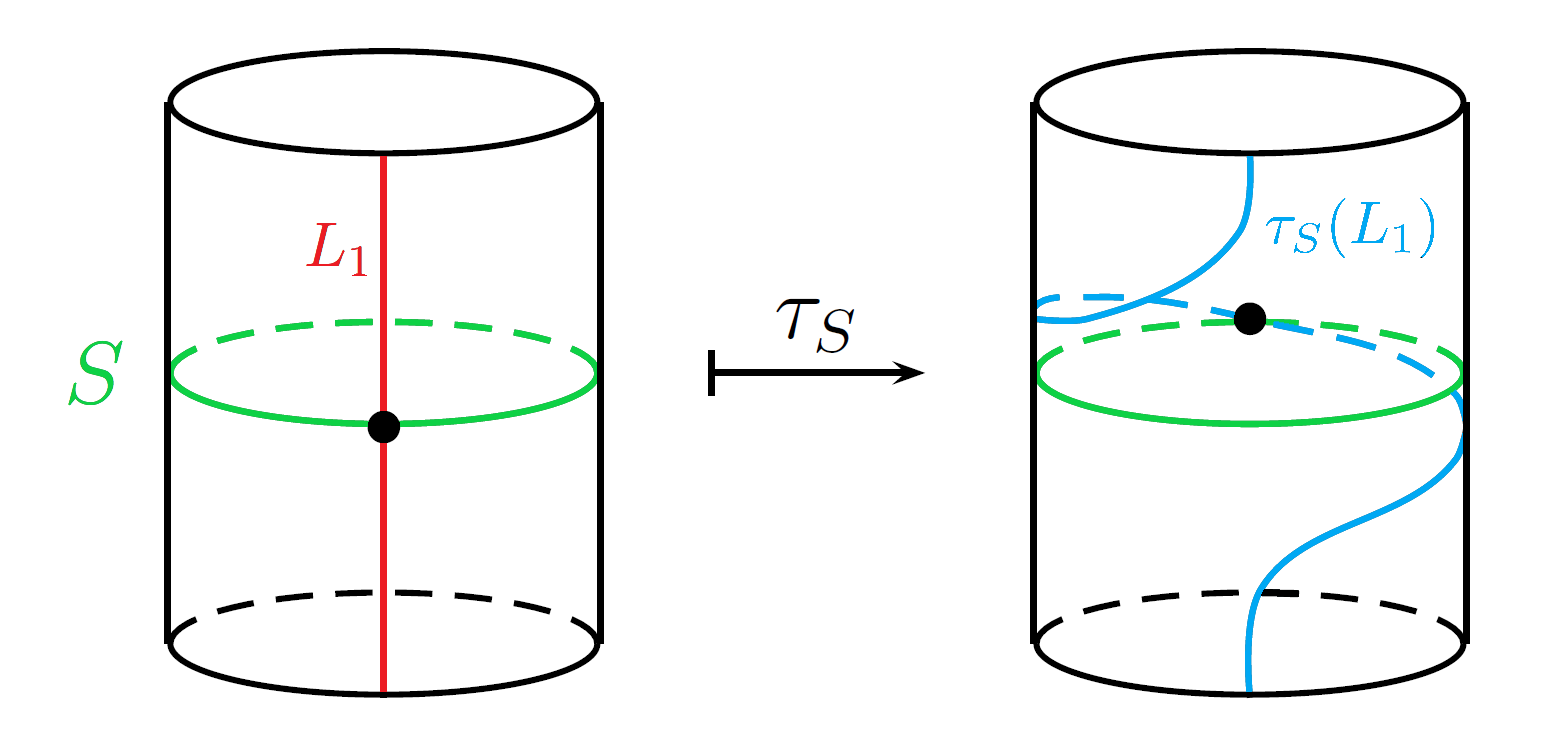
\includegraphics[width=0.8\linewidth]{fig10.png}
  \caption{沿球面 $S:=S_n$ 作用的 Dehn 扭转 $\tau_S$：所选纤维 $L_1$ 绕 $S$ 螺旋一周，并渐近地保持不变。\hfill（原书 p.100）}
  \label{fig:10}
\end{figure}

Dehn 扭转 $\tau_{S^n}$ 对 $T(\lambda)$ 的一条纤维的作用如图~\ref{fig:10} 所示。
有时便于通过要求 $h'|_{\mathbb R_{\ge0}}\ge0$、且只要“扭转速度” $h'$
超过某容差 $0<\varepsilon<1/2$ 就有 $h''<0$，来控制 $\tau_{S^n}$ 的
“摆动程度”。由此可以推断扭转后的纤维会在何处（横截地）与另一条未扭转的
纤维相交；若两条纤维的足点互为对径点，相交恰好发生在零截面上，正如图~\ref{fig:10}
所示（见 \cite{Sei02} 引理 1.9）。

我们把这一理论搬到流形层面。

\begin{Def}\label{def:6.22}
设 $M^{2n}=(M,\omega)$ 是辛流形。紧致拉格朗日子流形 $S^n\subset M$ 称为
\emph{拉格朗日球面}，若存在微分同胚 $f:S^n\to S$。它是\emph{标架的
（framed）}，若给定这样一些微分同胚的类 $[f]$，其中 $f_1\sim f_2$ 当且
仅当 $f_2^{-1}\circ f_1$ 可在 $\operatorname{Diff}(S^n)$ 内连续形变为
$O(n+1)$ 的某个正交矩阵。

对任意标架拉格朗日球面 $S=(S,[f])$ 可配一个 Dehn 扭转
$\tau_S\in\operatorname{Symp}(M,\omega)$。给定 $\lambda>0$，取任一代表
映射 $f:S^n\equiv T(0)\to S$ 并延拓到 $T(\lambda)$；后者经
$\iota:T(\lambda)\hookrightarrow M$ 辛嵌入 $M$，在 $T(\lambda)$ 内构造
支撑的 Dehn 扭转 \eqref{eq:6.90}。沿 $S$ 的 Dehn 扭转\footnote{读者不要被这里的记号迷惑：目前尚不知道
$[\tau_S]\in\pi_0(\operatorname{Symp}(M,\omega))$ 是否依赖于具体的类
$[f]$，尽管构造中其它所有选择实际上都无关紧要。为方便起见，我们不再
提及具体的标架 $[f]$，并隐含地把所有拉格朗日球面都视为已标架。}于是
为：
\begin{equation}
\tau_S(x):=
\begin{cases}
\iota\circ\tau_{S^n}\circ\iota^{-1}(x) & \text{若}\ x\in\operatorname{im}(\iota)\,,\\
x & \text{其它情形}\,.
\end{cases}
\label{eq:6.91}
\end{equation}
（具体地说，$\tau_S$ 是 $\phi^{2\pi}_H:M\setminus S\to M\setminus S$ 在
$S$ 上唯一可能的延拓，其中
$H:=h\circ\varrho\circ\iota^{-1}|_{\operatorname{im}(\iota)\setminus S}$
在 $M\setminus\operatorname{im}(\iota)$ 上为零。）特别地，$\tau_S$ 把
$S$ 对径地映到自身。
\end{Def}

% [Tutor Note: 【背景】定义 6.22 隐含使用了 Weinstein 拉格朗日邻域定理：
% 任何 $S\subset M$ 的邻域都辛同胚于 $T^*S^n$ 中零截面的邻域
% $T(\lambda)$。这正是可以把模型扭转 \eqref{eq:6.90} 搬到 $M$ 上的原因；
% 该定理见 \cite{Sil12} 定理 8.4。]

上一个定义隐含使用了 Weinstein 拉格朗日邻域定理（\cite{Sil12} 定理 8.4）：
$S\subset M$ 的任何邻域都辛同胚于 $S^n\equiv T(0)\subset T^*S^n$ 的
某个邻域 $T(\lambda)$（我们在命题 5.43 中也用过这一点）。

作为辛同胚，$\tau_S$ 把拉格朗日子流形映为拉格朗日子流形，并保持其全部
装饰（这一点并不平凡！）。换言之，$L\in\operatorname{obj}(\mathcal F(M))$
蕴含 $\tau_S(L)\in\operatorname{obj}(\mathcal F(M))$。我们关心的主要
结果是：

\begin{Thm}\label{thm:6.23}
设 $M$ 是辛流形，$\mathcal F(M)$ 是其相伴的 Fukaya 范畴。设
$S\in\operatorname{obj}(\mathcal F(M))$ 是拉格朗日球面，
$L\in\operatorname{obj}(\mathcal F(M))$ 是任意拉格朗日子流形。则
\begin{equation}
\tau_S(L)\cong T_S(L)=\operatorname{Cone}(\mathrm{ev})
\in\operatorname{obj}\bigl(\mathsf D^{\mathrm b}(\mathcal F(M))\bigr)\,,
\label{eq:6.92}
\end{equation}
其中 $T_S(L)$ 是 $L$ 沿 $S$ 的代数扭转，与
$\mathrm{ev}:CF(S,L)\otimes S\to L$ 的映射锥重合（如定义 4.21）。因此存在
正合三角形
\begin{equation}
\begin{tikzcd}[row sep=2.6em, column sep=3.4em]
HF(S,L)\otimes S \arrow[rr, "\langle \mathrm{ev}\rangle"] & & L \arrow[dl] \\
& \tau_S(L) \arrow[ul, "\langle\pi\rangle{[}1{]}"] \arrow[ur, "\langle c\rangle" swap] &
\end{tikzcd}
\label{eq:6.93}
\end{equation}
在 $\mathsf D^{\mathrm b}(\mathcal F(M))$ 中。于是，分别用
$HF(\tilde L,\square)$ 或 $HF(\square,\tilde L)$ 作用，给出长正合列
\[
\cdots\to\bigl(HF(S,L)\otimes HF(\tilde L,S)\bigr)^n
\xrightarrow{\langle\mu^2\rangle}HF^n(\tilde L,L)\to
HF^n(\tilde L,\tau_S(L))\xrightarrow{[1]}\cdots
\]
\[
\cdots\to HF^n(L,\tilde L)\to
\bigl(HF(S,L)\otimes HF(S,\tilde L)\bigr)^n
\xrightarrow{\langle d\rangle[1]}HF^{n+1}(\tau_S(L),\tilde L)\to\cdots
\]
对任意 $\tilde L\in\operatorname{obj}(\mathcal F(M))$ 成立；其中
$\mu^2$ 是 Floer 乘积，而 $\langle d\rangle$ 是一个复合，涉及典范同构
$HF(L,S)\cong HF(\tau_S(L),\tau_S(S))=HF(\tau_S(L),S)$ 与 Donaldson
“裤子”乘积。
\end{Thm}

\begin{proof}[证明（概要）]
这里只给出非常粗略的论证轮廓——精确证明是 Seidel 整篇论文
\cite{Sei02} 的内容。目标是先在 $A_\infty$-模层面工作，以便应用
引理 4.23。为保持一致，重记 $L_0:=S$、$L_1:=L$，并取
$L_2\in\operatorname{obj}(\mathcal F(M))$ 与 $\tau_{L_0}(L_1)$ 同痕；
由此定义 Floer 闭上链 $c\in CF(L_1,L_2)$（于是 $\mu^1(c)=0$）以及
$\mu^2(c,\,\cdot\,):CF(L_0,L_1)\to CF(L_0,L_2)$ 与零映射之间的链同伦
$k:CF(L_0,L_1)\to CF(L_0,L_2)[-1]$：
$\mu^1\circ k+k\circ\mu^1+\mu^2(c,\,\cdot\,)=0$。

在造出 \cite{Sei08} 引理 5.3 所需的适当附加数据之后（这在该书
(17d)--(17f) 各节中完成），引理 4.23 给出良定义的模同构
$t:T_{L_0}(\Upsilon(L_1))\to\Upsilon(L_2)$。还可改进此结果，把符号、
分次与膜结构一并纳入（\cite{Sei08} 定理 17.16）。因此
$T_{L_0}(\Upsilon(L_1))\cong\Upsilon(L_2)
\in\operatorname{obj}\bigl(H^0(\mathcal Q(M))\bigr)$。

现在借助注 4.22 第二个要点中的同构
$\mathcal T_{Y_0}(\tilde\Upsilon(Y_1))\cong
\tilde\Upsilon(\mathcal T_{Y_0}(Y_1))$ 过渡到扭复形。不妨设
$L_2=\tau_{L_0}(L_1)\in\operatorname{obj}(\operatorname{Tw}\mathcal F(M))$，
便得到
\[
\tilde\Upsilon(T_S(L))=\tilde\Upsilon(T_{L_0}(L_1))
\cong\mathcal T_{L_0}(\tilde\Upsilon(L_1))
\cong\tilde\Upsilon(\tau_{L_0}(L_1))=\tilde\Upsilon(\tau_S(L))\,,
\]
从而 $T_S(L)\cong\tau_S(L)\in\operatorname{obj}\bigl(\mathsf D^{\mathrm b}
(\mathcal F(M))\bigr)$（回忆 $\tilde\Upsilon$ 是拟等价）。

由图表 (89) 立即看出 $\tau_S(L)$ 嵌入正合三角形 \eqref{eq:6.93}；
其中我们辨认出 $c:L\to\tau_S(L)$ 恰是上面构造的 Floer 闭上链，而
$\langle\pi\rangle\in\hom_{\mathsf D^{\mathrm b}(\mathcal F(M))}
\bigl(\tau_S(L),(HF(S,L)\otimes S)[1]\bigr)\cong
\bigl(HF(S,L)\otimes HF(\tau_S(L),S)\bigr)^1\cong
\bigl(HF(S,L)\otimes HF(L,S)\bigr)^n$。此外，容易验证
$HF(\tilde L,\langle\mathrm{ev}\rangle)=\langle\mu^2\rangle$。关于 $d$
的确切定义，再次请读者参阅 \cite{Sei02}。
\end{proof}

% [Tutor Note: 【含糊】定理 6.23 的证明压缩了 Seidel 论文的整个主体：
% 链条是“$A_\infty$-模层面的模同构 $\Rightarrow$ 加符号/分次/膜结构
% $\Rightarrow$ 过渡到扭复形”。原文明确说精确证明是 \cite{Sei02} 的
% 内容，本译本不补。]

% [Tutor Note: 【易错】式 (92) 的 $\operatorname{Cone}(\mathrm{ev})$ 中
% $\mathrm{ev}:CF(S,L)\otimes S\to L$ 是“求值”态射，方向是
% $CF(S,L)\otimes S\to L$，不是反方向；相应的三角形 (93) 首项也因此写成
% $HF(S,L)\otimes S$。若把 $\mathrm{ev}$ 写成 $L\to CF(S,L)\otimes S$，
% 三个态射的次数都会错位。]

回顾扭映射锥通过 Yoneda 嵌入拟代表其抽象对应物，由定理 6.23 的证明还可
推出：

\begin{Cor}\label{cor:6.24}
设 $M$ 是辛流形，$\mathcal F(M)$ 是其相伴的 Fukaya 范畴。设
$S\in\operatorname{obj}(\mathcal F(M))$ 是拉格朗日球面，
$L\in\operatorname{obj}(\mathcal F(M))$ 是任意拉格朗日子流形。则 $L$ 沿
$S$ 的 Dehn 扭转 $\tau_S(L)\in\operatorname{obj}\bigl(\mathsf D^{\mathrm b}
(\mathcal F(M))\bigr)$ 拟代表 Yoneda 模
$\Upsilon(L)\in\operatorname{obj}(\mathcal Q(M))$ 沿 $S$ 的抽象代数扭转
$T_S(\Upsilon(L))\in\operatorname{obj}(\mathcal Q(M))$。
\end{Cor}

读者想必已经猜到，其背后的理论远比我们所触及的深刻——它围绕
Lefschetz 纤维化展开，而后者是 Picard--Lefschetz 理论的基本研究对象之一。
遗憾的是，详尽的研究超出我们的能力；感兴趣的读者可参阅 \cite{Sei08}
第三部分。

Fukaya 范畴的第二个有几何意义的侧面是所谓的\emph{拉格朗日手术}，其构造
在 \cite{FOOO07} 第 10.54 节中给出概要。先看另一件技术性准备。

\begin{Def}\label{def:6.25}
对满足 $|\varepsilon|>0$ 且足够小的 $\varepsilon\in\mathbb R$，考虑光滑
函数 $f_\varepsilon:\mathbb R^n\setminus\{0\}\to\mathbb R$，
$f_\varepsilon(x):=\varepsilon\log(\|x\|)$，以及它定义的 $1$-形式：
\[
df_\varepsilon(x)=\varepsilon\frac{x\cdot dx}{\|x\|^2}
=\sum_{j=1}^{n}y_j\,dx_j\in T^*_x(\mathbb R^n\setminus\{0\})\,,
\qquad y_j:=\varepsilon\frac{x_j}{\|x\|^2}\in\mathbb R\,.
\]
则 $H_\varepsilon:=\operatorname{graph}(df_\varepsilon)
=\{(x_1,y_1,\dots,x_n,y_n)\mid x\in\mathbb R^n\setminus\{0\}\}
\subset T^*(\mathbb R^n\setminus\{0\})\cong\mathbb C^n\setminus(i\mathbb R)^n$
是拉格朗日子流形，当 $\|x\|\to0$ 时渐近趋于 $(i\mathbb R)^n$（即
$0\in\mathbb R^n$ 上方的余切纤维），当 $\|x\|\to\infty$ 时渐近趋于零截面
$\mathbb R^n$；其中与复空间的等同由 $z_j:=x_j+iy_j\in\mathbb C$ 给出。

注意，若记 $r:\mathbb C^n\to\mathbb C^n$ 为沿对角线的反射
（$x_j+iy_j\mapsto y_j+ix_j$，$j=1,\dots,n$），则 $r(H_\varepsilon)
=H_\varepsilon$（事实上，构造的对称性说明 $H_\varepsilon$ 也是镜像图像，
由一切满足 $y\in\mathbb R^n\setminus\{0\}$ 且
$x_j=\varepsilon y_j/\|y\|^2$ 的 $(y_1,x_1,\dots,y_n,x_n)\in
T^*(\mathbb R^n\setminus\{0\})$ 组成）。

再取修正用的光滑函数 $g\in C^\infty(\mathbb R_{>0})$，使得当
$0<x\le x_0$ 时 $g(x)=\log(x)-|\varepsilon|$，其中
$x_0\equiv x_0(|\varepsilon|)$ 足够小；当 $x\ge 2x_0$ 时 $g$ 为常数，
且 $g'\ge0$、$g''\le0$（与引理 6.20 中的映射 $h$ 比较）。定义调整后的
光滑函数
\[
\tilde f_\varepsilon:\mathbb R^n\setminus\{0\}\to\mathbb R\,,\qquad
\tilde f_\varepsilon(x):=\varepsilon g(\|x\|)=
\begin{cases}
f_\varepsilon(x)-\varepsilon|\varepsilon| & \text{若}\ 0<x\le x_0\,,\\
\text{常数} & \text{其它情形}\,,
\end{cases}
\]
并考察其图像 $\tilde H_\varepsilon:=\operatorname{graph}(d\tilde f_\varepsilon)
\subset T^*(\mathbb R^n\setminus\{0\})$；它仍是拉格朗日子流形，且在反射
$r$ 下不变。特别地，在 $0$ 处半径为 $2x_0$ 的 $n$ 维复球
$B^n_{2x_0}(0)\subset\mathbb C^n$ 之外，
$\tilde H_\varepsilon=\mathbb R^n\cup(i\mathbb R)^n$。
\end{Def}

% [Tutor Note: 【易错】$f_\varepsilon=\varepsilon\log\|x\|$ 的符号决定
% 手术“从哪一侧”光滑化：$H_\varepsilon$ 在 $\|x\|\to0$ 时贴到余切纤维
% $(i\mathbb R)^n$ 上、在 $\|x\|\to\infty$ 时贴到零截面 $\mathbb R^n$ 上。
% 因此 $L_1\#_\varepsilon L_2=L_2\#_{-\varepsilon}L_1$：交换次序必须同时
% 把 $\varepsilon$ 变号。这正是后文强调 $L_2\#_\varepsilon L_1$ 连同痕
% 都不对的原因。]

\begin{Def}\label{def:6.26}
设 $M^{2n}=(M,\omega)$ 是辛流形，$\mathcal F(M)$ 是其相伴的 Fukaya 范畴。
设 $L_1,L_2\in\operatorname{obj}(\mathcal F(M))$ 在某个 $p\in M$ 处横截
相交。取适当的 Darboux 坐标卡\footnote{这是局部坐标
$(x^j,y^j)_{j=1}^n$，使 $\omega|_U=\sum_{j=1}^n dx^j\wedge dy^j$；
由 \cite{Sil12} 定理 8.1，这样的坐标卡总是存在。}
$\psi:U\subset M\to V\subset\mathbb R^{2n}\cong\mathbb C^n$，定义在 $p$
的邻域 $U$ 上、以 $p$ 为中心（故 $\psi(p)=0$）；可把两条拉格朗日子流形
摆成 $\psi(L_1\cap U)=\mathbb R^n\cap V$ 与
$\psi(L_2\cap U)=(i\mathbb R)^n\cap V$。

现在按定义 6.25 构造 $\tilde H_\varepsilon$，并调整 $\varepsilon$ 使
$B^n_{2x_0}(0)\subset\psi(U)$。于是
\begin{equation}
L_1\#_\varepsilon L_2:=
\begin{cases}
(L_1\cup L_2)\setminus U & \text{在}\ M\setminus U\ \text{上}\,,\\
\psi^{-1}(\tilde H_\varepsilon)\cap U & \text{在}\ U\ \text{上}\,,
\end{cases}
\label{eq:6.94}
\end{equation}
称为 $L_1$ 与 $L_2$ 在 $p$ 处的\emph{拉格朗日连通和}（或\emph{拉格朗日
手术}），有时简记为 $L_1\#L_2$。它是 $M$ 的拉格朗日子流形，继承全部
所需的装饰（这一点并不平凡！），即 $L_1\#_\varepsilon L_2
\in\operatorname{obj}(\mathcal F(M))$。区域
$(L_1\#_\varepsilon L_2)\cap U=\psi^{-1}(\tilde H_\varepsilon)\cap U$
称为\emph{拉格朗日把手}。
\end{Def}

二维情形如图~\ref{fig:11} 所示，四维情形可参阅 \cite{AS09} 第 3 节。

由上述构造可知 $L_1\#_\varepsilon L_2=L_2\#_{-\varepsilon}L_1$（而不是
$L_2\#_\varepsilon L_1$，后者甚至不同痕于 $L_1\#_\varepsilon L_2$！）。
此外，只要 $\operatorname{sgn}(\varepsilon)=\operatorname{sgn}(\delta)$，
$L_1\#_\varepsilon L_2$ 就哈密顿同痕于某个 $L_1\#_\delta L_2$（在拉格朗日
把手的适当管状邻域中计算即可看出）。然而，若在多个不同点作手术，最终
结果就失去同痕不变性。

% [Tutor Note: 【含糊】“在拉格朗日把手的适当管状邻域中计算”省略了
% $L_1\#_\varepsilon L_2$ 与 $L_1\#_\delta L_2$ 之间的显式哈密顿同痕；
% 其要点是把 $\varepsilon$ 连续形变到同号的 $\delta$（保持
% $|\varepsilon|>0$ 足够小），并让调整函数 $g$ 随之连续变化。]

\begin{figure}[htbp]
  \centering
  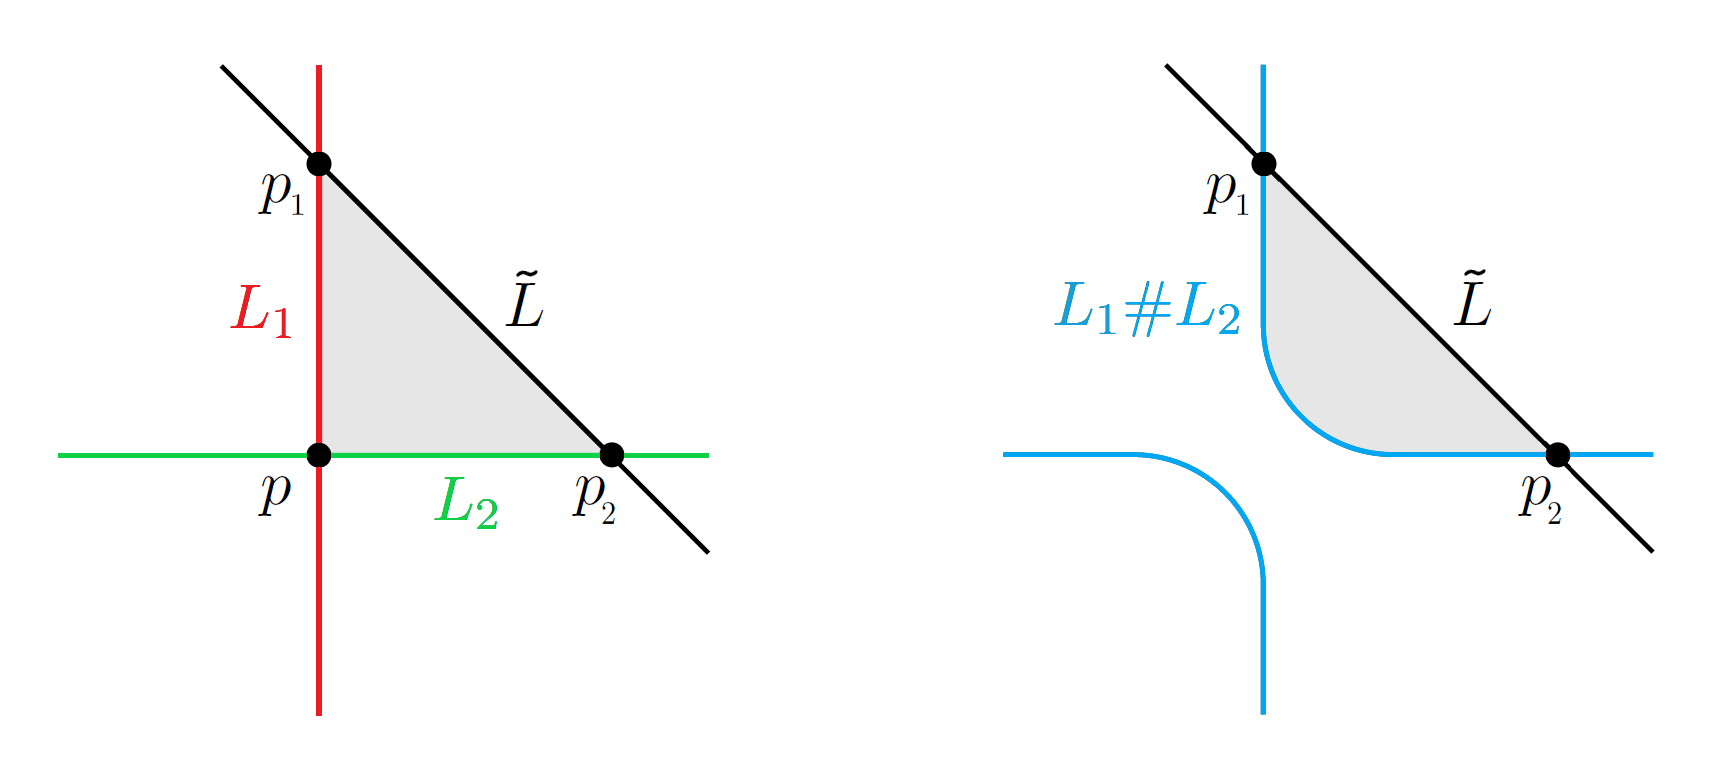
\includegraphics[width=0.8\linewidth]{fig11.png}
  \caption{两个一维拉格朗日子流形 $L_1,L_2\subset M^2$ 在 $p\in M$ 处横截相交时的拉格朗日连通和 $L_1\#L_2$；在 $0\in\mathbb C$ 的某个邻域内，经适当的 Darboux 坐标卡，它们分别映为实轴与虚轴。$L_1\#L_2$ 的“弯曲区域”即所谓的拉格朗日把手。\hfill（原书 p.103）}
  \label{fig:11}
\end{figure}

\begin{Rem}\label{rem:6.27}
取 $L_2=S\in\operatorname{obj}(\mathcal F(M))$ 为拉格朗日球面，与 $L_1$
在唯一一点 $p$ 处横截相交。则 $L_1\#S$ 哈密顿同痕于 Dehn 扭转
$\tau_S(L_1)$：
\begin{equation}
L_1\#S\simeq\tau_S(L_1)
\label{eq:6.95}
\end{equation}
（与图~\ref{fig:10} 比较）。因此，$S$ 调控扭转，而 $L_1$ 支配渐近行为。在二维情形，
$L_1$ 的局部 Darboux 图像对应虚直线 $i\mathbb R$，$S$ 的局部图像对应以
$1\in\mathbb C$ 为圆心的 $S^1$。于是拉格朗日手术相当于把 $S^1$ 与
$i\mathbb R$ 之间在 $0$ 附近被挤压的角形区域磨光。这可非正式地看作产生
拉格朗日连通和的一般配方。
\end{Rem}

% [Tutor Note: 【易错】式 (95) 中 $\simeq$ 表示哈密顿同痕，而非同构；
% $L_1\#S$ 与 $\tau_S(L_1)$ 只是同痕的拉格朗日子流形，在 $\mathcal F(M)$
% 的上同调范畴中才成为同构对象。原文在此用了 $\simeq$ 而非 $\cong$，
% 译文保留这一区别。]

与 Dehn 扭转类似，拉格朗日连通和与扭映射锥密切相关：

\begin{Thm}\label{thm:6.28}
设 $L_1,L_2\in\operatorname{obj}(\mathcal F(M))$ 在唯一一点 $p\in M$ 处
横截相交，于是 $p$ 必然是 $CF(L_2,L_1)$ 的 Floer 闭上链。\footnote{这由
Floer 复形与微分的定义立得：$\mu^1$ 是 $1$ 次的，故不可能保持
$\mathcal X(L_2,L_1)$ 中唯一的生成元 $p$。}再取第三条
$\tilde L\in\operatorname{obj}(\mathcal F(M))$，使交点满足
$\tilde L\cap(L_1\#_\varepsilon L_2)=(\tilde L\cap L_1)\cup
(\tilde L\cap L_2)$（当 $|\varepsilon|$ 足够小时可行；参看图~\ref{fig:11}）。记
$p_i$ 为 $\tilde L\cap L_i$ 中的横截交点。则对由 $\tilde L$ 与
$L_1\#_\varepsilon L_2$ 所围区域上适当的近复结构
$J\in\mathcal J(M,\omega)$，存在双射
\[
\left\{\begin{array}{c}
\text{以}\ \tilde L\ \text{与}\ L_1\#_\varepsilon L_2\ \text{为边界}\\
\text{从}\ p_2\ \text{到}\ p_1\ \text{的}\ J\text{-全纯条带}
\end{array}\right\}
\longleftrightarrow
\left\{\begin{array}{c}
\text{以}\ \tilde L,L_1,L_2\ \text{为边界，从}\ p_2\ \text{经}\ p_1\\
\text{到}\ p\ \text{的}\ J\text{-全纯三角形}
\end{array}\right\}.
\]
作为推论，$CF(\tilde L,L_1\#_\varepsilon L_2)$ 是
$\mu^2(p,\,\cdot\,):CF(\tilde L,L_2)\to CF(\tilde L,L_1)$ 的标准映射锥
（在上链复形意义下），于是嵌入短正合列
\[
\{0\}\to CF(\tilde L,L_1)\to CF(\tilde L,L_1\#_\varepsilon L_2)
\to CF(\tilde L,L_2)\to\{0\}\,,
\]
它诱导长正合列
\begin{equation}
\begin{aligned}
\cdots\to HF^n(\tilde L,L_1)&\to HF^n(\tilde L,L_1\#_\varepsilon L_2)
\to HF^n(\tilde L,L_2)\\
&\xrightarrow{\langle\mu^2(p,\,\cdot\,)\rangle[1]}\cdots\,.
\end{aligned}
\label{eq:6.96}
\end{equation}
事实上存在正合三角形
\begin{equation}
\begin{tikzcd}[row sep=2.6em, column sep=3.4em]
L_2 \arrow[rr, "\langle p\rangle"] & & L_1 \arrow[dl] \\
& L_1\#_\varepsilon L_2 \arrow[ul, "\langle\pi\rangle{[}1{]}"] \arrow[ur, "\langle i\rangle" swap] &
\end{tikzcd}
\label{eq:6.97}
\end{equation}
在 $\mathsf D^{\mathrm b}(\mathcal F(M))$ 中，也就是说
\begin{equation}
L_1\#_\varepsilon L_2\cong\operatorname{Cone}(p)
\in\operatorname{obj}\bigl(\mathsf D^{\mathrm b}(\mathcal F(M))\bigr)\,.
\label{eq:6.98}
\end{equation}
\end{Thm}

% [Tutor Note: 【易错】三角形 (97) 的方向是 $L_2\xrightarrow{\langle p\rangle}L_1
% \xrightarrow{\langle i\rangle}L_1\#_\varepsilon L_2$，即映射锥的“第一项”
% 是 $L_2$ 而不是 $L_1$；这与 (98) 中 $\operatorname{Cone}(p)$ 的次序一致。
% 若把 $p$ 看成 $CF(L_1,L_2)$ 的元素，三角形要整体反向，易生混淆。]

该结果的证明贯穿 \cite{FOOO07} 第 10.59--10.62 节（那里称之为
“定理 Z”）。为研究由 $L_1\#_\varepsilon L_2$ 与 $\tilde L$ 界定的
$J$-全纯条带所对应的模空间
$\mathcal M(p_2,p_1;[u],J,H)$，该证明大量依赖我们在第 5 章偶尔提及的
分析工具以及粘接技巧，并利用了复空间 $\mathbb C^n$ 中的局部构造。

\begin{Rem}\label{rem:6.29}
仍取 $L_2=S\in\operatorname{obj}(\mathcal F(M))$ 为拉格朗日球面，使
$L_1\#S\simeq\tau_S(L_1)$。于是定理 6.28 的断言与定理 6.23 的断言相容。
事实上，把连接同态
$\langle\mu^2\rangle:HF(S,L_1)\otimes HF(\tilde L,S)\to HF(\tilde L,L_1)$
的输入固定为 $\langle p\rangle\in HF(S,L_1)$（并重记 $L:=L_1$）之后，
\eqref{eq:6.93} 诱导的长正合列正是 \eqref{eq:6.96}。同样，图表
\eqref{eq:6.93} 取 \eqref{eq:6.97} 的形状。
\end{Rem}

最后提醒一点：把 Dehn 扭转与拉格朗日连通和等同于扭映射锥，是一把双刃剑：
代数对象与几何对象之间这种词典的好处，部分被处理高阶 Floer 复合映射
$\mu^d$ 的必要性所抵消——想想作多次手术时图~\ref{fig:11} 的局部图像。因此，
研究拉格朗日构件（constituents）不可避免地要求我们增强手头的分析工具。
这超出本书范围；我们不再深入。

最后给出关于分裂封闭 $\mathsf D^\pi(\mathcal F(M))$ 之重要性的一些启发。
给定有限多条拉格朗日子流形 $L_i\in\operatorname{obj}(\mathcal F(M))$，
它们生成 $A_\infty$-子范畴 $\mathcal A\subset\mathcal F(M)$；则
$A_\infty$-范畴 $\operatorname{Tw}\mathcal A$ 包含由它们迭代可构造的
一切映射锥，特别是 Dehn 扭转与拉格朗日连通和。对全部初始对象作手术，
可能产生一条不连通的拉格朗日子流形。它虽是 $\mathcal A$ 的元素，其连通
分支却未必还是 $\mathcal A$ 的元素。因此人们猜想：取
$\operatorname{Tw}\mathcal A$ 的幂等完备化，可以把各个构件作为
$\mathsf D^\pi(\mathcal A)$ 的对象纳入，从而弥补这一缺陷。在环面的情形，
这一点尤其成立：

\begin{Ex}\label{ex:6.30}
考虑辛环面 $\mathbb T^2=S^1\times S^1$，配以标准面积形式
$\omega:=d\theta_1\wedge d\theta_2$，其中 $\theta_1$ 与 $\theta_2$ 是
相应因子 $S^1\subset\mathbb C$ 上的角坐标。\footnote{注意
$\theta_j(e^{2\pi it}):=t\in(0,1)$ 只在 $S^1\setminus\{1\}$ 上良定义，
并非整体定义，因此 $d\theta_j$ 并非由 $\theta_j$ 的外微分所得的
$1$-形式！}$\mathcal F(\mathbb T^2)$ 的对象（即带装饰的拉格朗日子流形）
是 $\mathbb T^2$ 上的一切\emph{简单环路}（即不自交的闭道路），可等同于
$\mathbb Z\oplus\mathbb Z=\pi_1(\mathbb T^2)$ 的类代表元，并由其在
$\mathbb T^2$ 的商空间表示中的有理斜率（同伦意义下）决定。

取定一条经线方向的环路 $L_1:=\alpha\in\operatorname{obj}(\mathcal F(\mathbb T^2))$
与一条纬线方向的环路 $L_2:=\beta\in\operatorname{obj}(\mathcal F(\mathbb T^2))$，
它们分别沿着 $\mathbb T^2$ 的等同多边形的两个因子（图~\ref{fig:12} 左上）；它们
属于 $\pi_1(\mathbb T^2)$ 的类 $(1,0)$ 与 $(0,1)$。记
$p\in CF(L_2,L_1)$ 为 $\alpha$ 与 $\beta$ 的唯一交点。由于 $\beta$
显然微分同胚于 $S^1$，它是拉格朗日球面，故可构造 $\alpha$ 沿它的 Dehn
扭转。由注 6.27 与定理 6.28，这给出新的简单环路
$\tau_\beta(\alpha)\simeq\alpha\#\beta\cong\operatorname{Cone}(p)
\in\operatorname{obj}\bigl(\mathsf D^{\mathrm b}(\mathcal F(\mathbb T^2))\bigr)$，
如图~\ref{fig:12} 右上所示。Dehn 扭转过程可以无限迭代（这相当于第 4.4 节所讨论的
反复取代数扭转），并同样可沿 $\alpha$ 施加 $\tau_\alpha$。

由于我们将遍历 $\pi_1(\mathbb T^2)$ 的所有同伦类——事实上
$\tau_\alpha,\tau_\beta\in\operatorname{Diff}(\mathbb T^2)$ 生成
$\mathbb T^2$ 的映射类群，即其微分同胚的环境同痕类——人们自然会期待
由此得到 $\mathcal F(\mathbb T^2)$ 的全部对象；但事实远非如此：取
$\nu\in\Omega^1(\mathbb T^2\setminus\{p\})$ 使 $d\nu=\omega$
（在挖去一点的环面上这是可行的），且
$\int_\alpha\nu=\int_\beta\nu=0$，这意味着
$\alpha,\beta\subset\mathbb T^2$ 是\emph{平衡的}（或\emph{正合的}）
拉格朗日子流形，且 $\nu|_\alpha=d\theta_\alpha$、$\nu|_\beta=d\theta_\beta$
（于是确实 $\int_\alpha\nu=\int_\alpha d\theta_\alpha
=\theta_\alpha(e^{2\pi i})-\theta_\alpha(e^0)=0$，对 $\beta$ 同理）。
那么上面构造的一切后续映射锥也将是正合的：观察图~\ref{fig:12} 左上中的
$\tau_\beta(\alpha)$，可见它在 $[0,1]\times[0,1]$ 上的双射性使其所描述的
Dehn 扭转后的拉格朗日子流形为正合——换个说法，若沿相应的简单环路追踪
（见图~\ref{fig:12}），会看到它绕每个因子恰好一周（事实上
$\tau_\beta(\alpha)$ 代表 $(1,1)\in\pi_1(\mathbb T^2)$）。这显然是我们
需要去除的限制，因为并非所有简单环路都正合！

\begin{figure}[htbp]
  \centering
  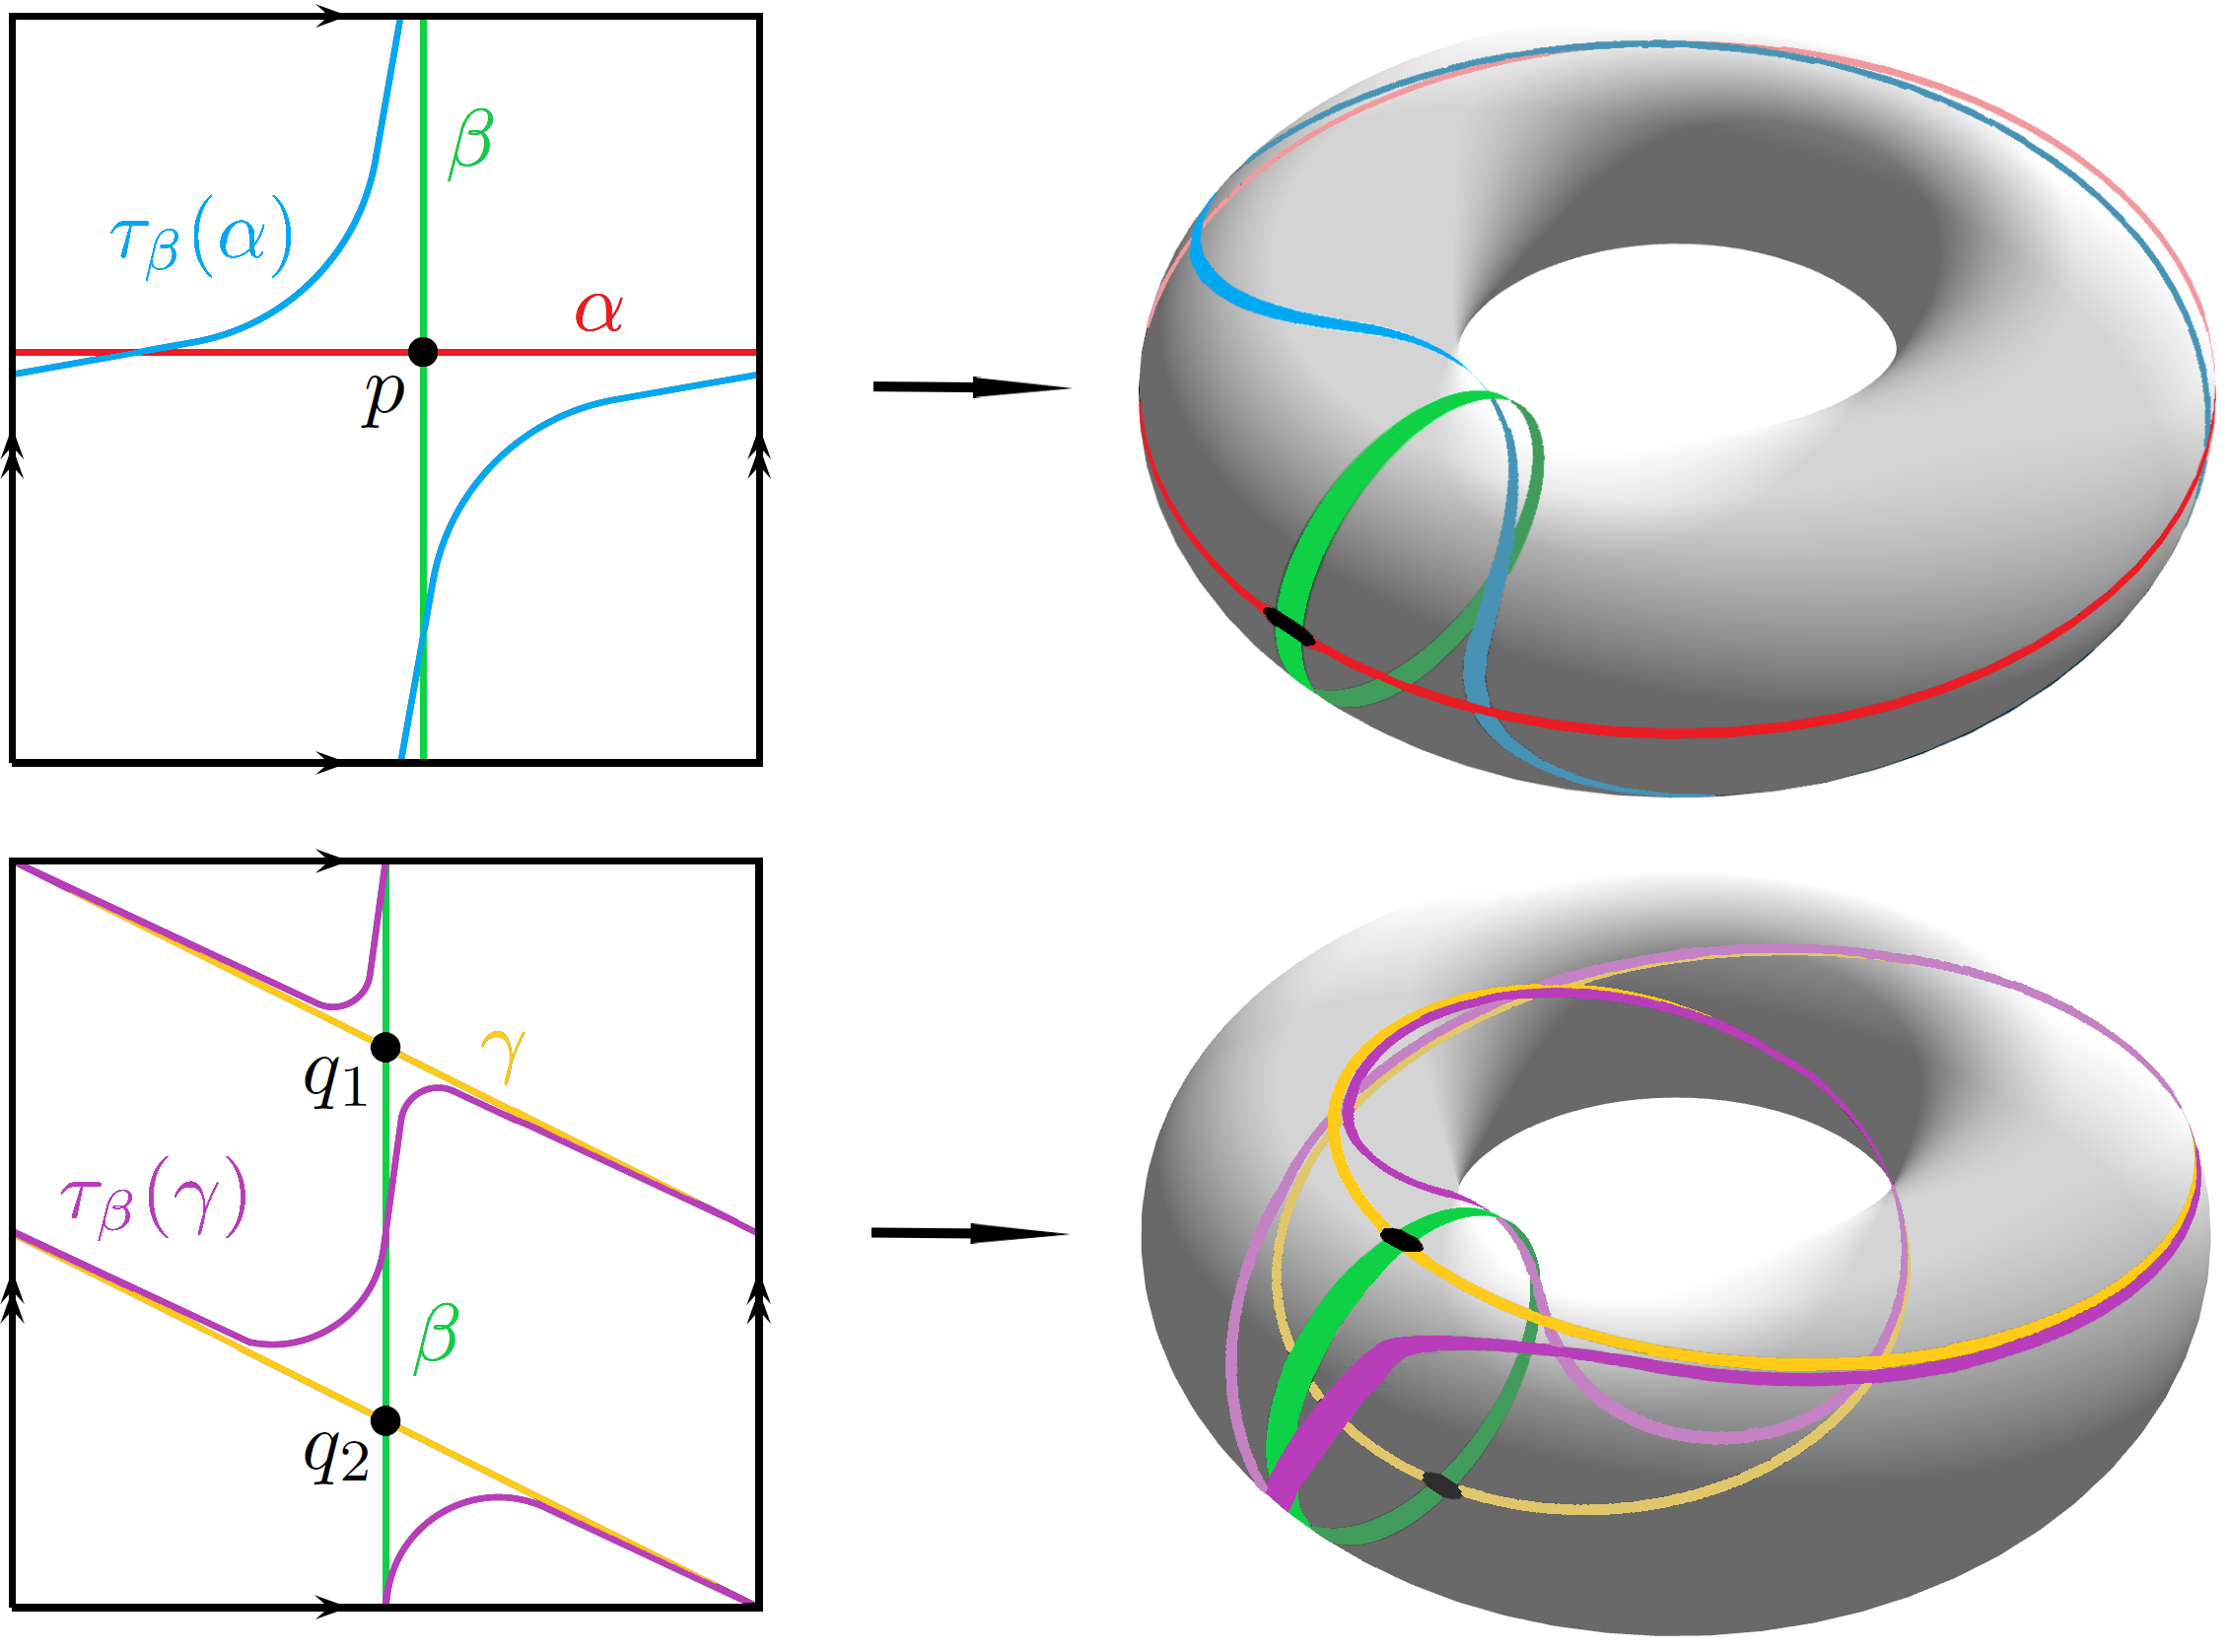
\includegraphics[width=0.85\linewidth]{fig12.png}
  \caption{两个简单闭曲线的拉格朗日连通和可能给出非平衡简单闭曲线的直和（下排）。它们是分裂封闭导出范畴 $\mathsf D^\pi(\mathcal F(T^2))$ 的真正对象。\hfill（原书 p.106）}
  \label{fig:12}
\end{figure}

例如，考虑第三条简单环路
$L_3:=\gamma\in\operatorname{obj}(\mathcal F(\mathbb T^2))$，其有理斜率为
$-1/2$（图~\ref{fig:12} 左下），代表类 $(2,1)\in\pi_1(\mathbb T^2)$（即
$\tau_\alpha(\tau_\alpha(\beta))$ 的类）；它与 $\beta$ 相交两次，设交点为
$q_1,q_2\in CF(L_2,L_3)$。构造 $\gamma$ 与 $\beta$ 的（二重）连通和，
并小心应用定理 6.28，可得
$\tau_\beta(\gamma)\simeq\gamma\#\beta
\cong\operatorname{Cone}(T^{w_1}q_1+T^{w_2}q_2)$ 在
$\mathsf D^{\mathrm b}(\mathcal F(\mathbb T^2))$ 中成立，其中权重
$w_1,w_2\in\mathbb R$ 适当。其几何结果恰是图~\ref{fig:12} 右下那两条紫色的、
非正合简单环路之直和，它们都落在 $\alpha$ 的同伦类 $(1,0)$ 中。用心的
读者已经知道下一步：取 $\mathcal F(\mathbb T^2)$ 的分裂封闭，从而把
映射锥的两个直和项都作为 $\mathsf D^\pi(\mathcal F(\mathbb T^2))$ 的
对象纳入。

总之，通过沿 $\alpha$ 与 $\beta$ 反复扭转并最终纳入出现的直和项，可以
得到 $\mathbb T^2$ 的一切简单环路（在哈密顿同痕意义下）。更系统的讨论见
\cite{LP11}，尤其侧重拉格朗日手术与由此产生的正合三角形。我们的处理旨在
为下一个结果提供几何直观。
\end{Ex}

% [Tutor Note: 【易错】$\operatorname{Cone}(T^{w_1}q_1+T^{w_2}q_2)$ 中
% 的 $T^{w_i}$ 是 Novikov 系数（$T$ 是 Novikov 变量），权重
% $w_1,w_2\in\mathbb R$ 来自两条条带的辛面积；它不是拓扑对象，而是
% 打点计数中的指数权。若把 $T^{w_i}$ 误读为“$T$ 的 $w_i$ 次幂算子”，
% 会误以为这是某种几何运算。]

\begin{Pro}\label{pro:6.31}
辛 $2$-环面 $\mathbb T^2=S^1\times S^1$ 的任意一对经线与纬线都分裂生成
其 Fukaya 范畴 $\mathcal F(\mathbb T^2)$。因此，任何微分同胚于
$\mathbb T^2$ 的紧致 $2$ 维辛流形 $M^2$，其 Fukaya 范畴 $\mathcal F(M)$
都被任意一对经线与纬线同构地分裂生成。
\end{Pro}

\begin{proof}[证明（概要）]
我们直接在 $M$ 上工作。设 $S_1,S_2\in\operatorname{obj}(\mathcal F(M))$
分别微分同胚于上一例中固定的经线与纬线。取任一同伦本质的闭曲线（即
$\mathbb T^2$ 中简单环路的流形类比）。我们要证明它落在 $\{S_1,S_2\}$
的分裂封闭中，于是整个 Fukaya 范畴 $\mathcal F(M)$ 也如此。

首先可以证明，对所有 $k\ge1$ 都有
$(\tau_{S_1}\circ\tau_{S_2})^{6k}=1\in SL(2,\mathbb Z)$。于是存在典范
态射 $i:L\to(\tau_{S_1}\circ\tau_{S_2})^{6k}(L)\cong L$，它嵌入
$\mathsf D^{\mathrm b}(\mathcal F(M))$ 中的图表
\[
\begin{tikzcd}[row sep=2.6em, column sep=3.6em]
Y \arrow[rr] & & L \arrow[dl, "\langle i\rangle"] \\
& (\tau_{S_1}\circ\tau_{S_2})^{6k}(L) \arrow[ul] &
\end{tikzcd}
\]
其中由三角范畴的公理 (T1)，可找到某个
$Y\cong\operatorname{Cone}(i)\in\operatorname{obj}\bigl(\mathsf D^{\mathrm b}
(\mathcal F(M))\bigr)$ 补全正合三角形。注意由命题 5.43，
$\langle i\rangle\in HF^0(L,L)\cong H^0(L)$ 只是一个奇异上同调类。
若它为零，则由注 3.48 的讨论立即推出
$\operatorname{Cone}(i)\cong L\oplus L$，从而 $L$ 是一个直和项，必被纳入
$\{S_1,S_2\}$ 的分裂封闭中，正如所断言。

可以证明，若取 $k=2$，则 $\langle i\rangle=0$。然而其背后的论证对我们
所发展的有限工具而言过于曲折。读者可参阅 \cite{AS09} 命题 6.1 以了解
主要策略的概要。
\end{proof}

% [Tutor Note: 【含糊】“对所有 $k\ge1$ 有 $(τ_{S_1}∘τ_{S_2})^{6k}=1\in SL(2,Z)$”
% 依赖映射类群 $MCG(\mathbb T^2)=SL(2,\mathbb Z)$ 中两个 Dehn 扭转生成元
% 的关系 $(\tau_\alpha\tau_\beta)^6=1$；原文未给证明。取 $k=2$ 时
% $\langle i\rangle=0$ 更只是引用 \cite{AS09} 命题 6.1，本译本不补写。]

\subsection{wrapped Fukaya 范畴}\label{sec:6.5}

作为本章的结束，我们简要而颇为含糊地讨论 Fukaya 范畴的 wrapped 版本，
它处理正合辛流形（回忆第 5.8 节的设定）。其主要优点是：我们不再需要
要求正合拉格朗日子流形紧致，只需其在无穷远处有某种行为。我们仍按
\cite{Aur13} 第 4.1 节的纲要进行，并参照 \cite{Abo10} 第 2 节。先补充
一些工作工具（见 \cite{Sil12}）。

\begin{Def}\label{def:6.32}
设 $M^n$ 是光滑流形。点 $p\in M$ 称为\emph{接触点}，若它有一个切超平面
$H_p\subset T_pM$，即维数为 $\dim(H_p)=n-1$ 的子空间。

给定光滑截面 $H\in\Gamma(TM)$（\emph{接触分布}），$p\mapsto H_p$；
局部可写作 $H=\ker(\alpha)$，其中 $\alpha\in\Omega^1(M)$ 不唯一，且
$d\alpha|_H$ 是辛形式。于是每个 $H_p$ 都是某个线性映射
$0\neq\alpha_p:T_p\to\mathbb R$ 的核。我们称 $\alpha$ 为 $M$ 上的
\emph{接触形式}。其非退化性迫使 $M$ 的维数 $n$ 为奇数。
\end{Def}

\begin{Def}\label{def:6.33}
正合辛流形 $M^{2n}=(M,\omega)$（$\omega=d\lambda\in\Omega^2(M)$）称为
\emph{Liouville 流形}，若它配有某个完备的 $Z\in\mathfrak X(M)$，该向量场
在无穷远处向外（见下一段），并满足 $\iota_Z(\omega)=\lambda$，或等价地
$\mathcal L_Z(\omega)=\omega$。此时 $Z$ 称为与 Liouville 形式
$\lambda\in\Omega^1(M)$ 相伴的\emph{Liouville 向量场}。
\end{Def}

我们特别关心这样的 Liouville 流形 $(M^{2n},\omega=d\lambda)$：它含有某个
紧致区域 $M^{in}\subset M$，具有如下性质（见图~\ref{fig:13}）：
\begin{itemize}
  \item $(2n-1)$ 维边界 $\partial M^{in}$ 是光滑超曲面，配有接触形式
  $\alpha:=\lambda|_{\partial M^{in}}\in\Omega^1(\partial M^{in})$；
  \item $\operatorname{zeros}(Z)\subset M^{in}$，且 $Z$ 正横截于
  $\partial M^{in}$，即对一切 $x\in\partial M^{in}$ 有
  $Z(x)\notin T_x(\partial M^{in})$ 且 $Z(x)(x^1)>0$（在 $x$ 周围的适当
  半空间坐标卡中）。
\end{itemize}

$Z$ 的流 $\phi^t_Z:M\to M$ 使我们能把 $M\setminus M^{in}$ 等同于
辛化 $[1,\infty)\times\partial M^{in}$：其中给定径向坐标函数
$r\in C^\infty([1,\infty))$，有
$Z=r\frac{\partial}{\partial r}$ 与 $\lambda=r\alpha$。滥用记号，我们可以
非正式地把 Liouville 流形写成粘合空间
\begin{equation}
M=M^{in}\sqcup_{\partial M^{in}}\bigl([1,\infty)\times\partial M^{in}\bigr)\,.
\label{eq:6.99}
\end{equation}
为后文之用，记 $\psi^\rho_Z:=\phi^{\log\rho}_Z$ 为 $Z$ 的时间
$\log\rho$ 流（$\rho>1$）；注意 $\phi^t_Z$ 是共形辛的，故
$\psi^\rho_Z\in\operatorname{Symp}(M,\omega)$。

% [Tutor Note: 【易错】$M\setminus M^{in}\cong[1,\infty)\times\partial M^{in}$
% 中的坐标 $r$ 满足 $Z=r\,\partial/\partial r$、$\lambda=r\alpha$；因此
% 时间 $t$ 的流把 $r$ 变成 $e^t r$，从而 $\psi^\rho_Z=\phi^{\log\rho}_Z$
% 把 $r$ 乘以 $\rho$。这个“时间–半径”对应在定义 $\mu^2_{W(M)}$ 的
% 重标度（$\rho=2$）时反复用到。]

\begin{figure}[htbp]
  \centering
  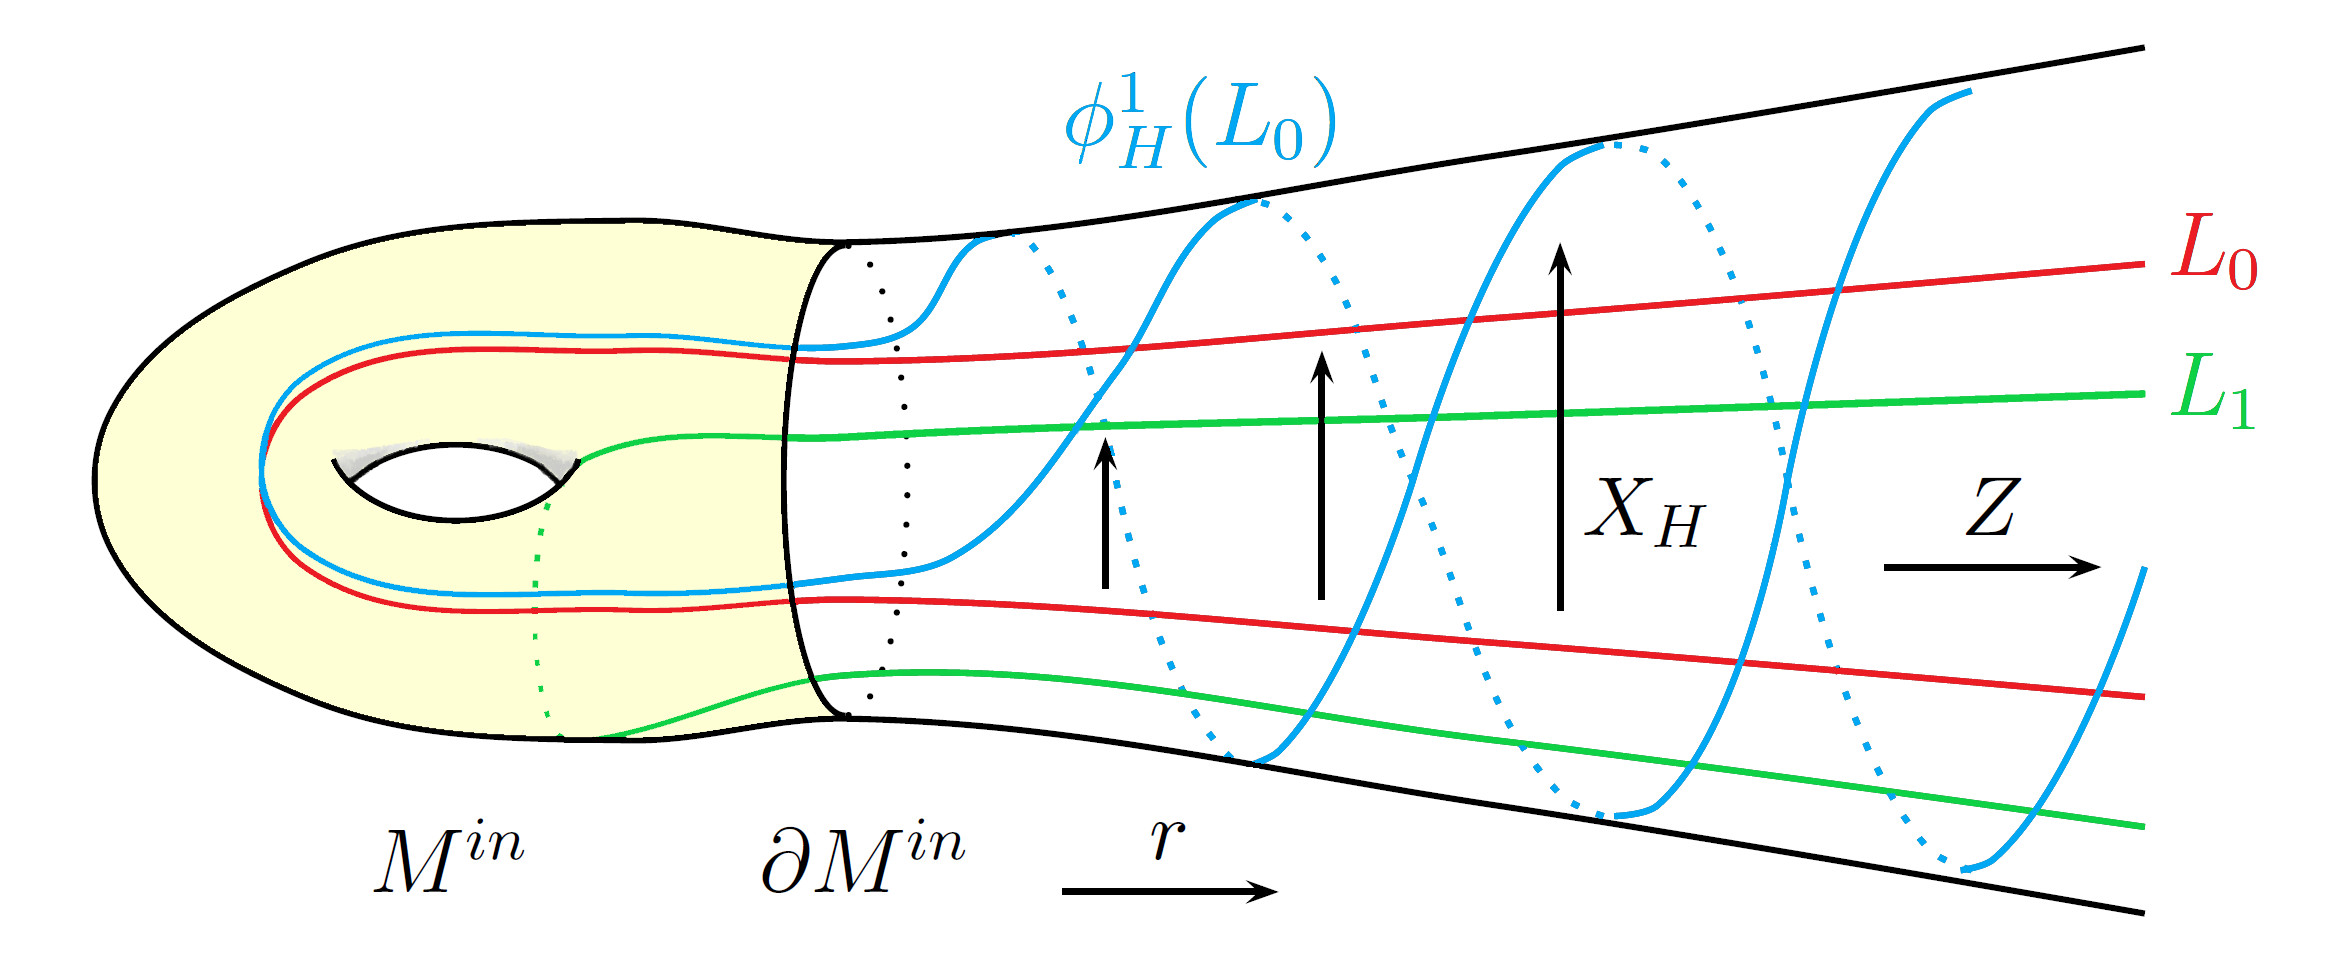
\includegraphics[width=0.8\linewidth]{fig13.png}
  \caption{Liouville 二维流形 $M$ 的正合拉格朗日子流形 $L_0,L_1\in\operatorname{obj}(\mathcal W(M))$。“卷绕哈密顿量” $H\in C^\infty(M)$（在 $M$ 的某紧子集之外为二次型）的流使 $L_0$ 沿径向向外螺旋。\hfill（原书 p.108）}
  \label{fig:13}
\end{figure}

给定如上所述的 Liouville 流形 $(M^{2n},\omega=d\lambda)$（且
$2c_1(TM)=0$），其 \emph{wrapped Fukaya 范畴} $\mathcal W(M)$ 是如下
构造的 $A_\infty$-范畴（更从容的探讨见 \cite{Abo10}）：

\begin{itemize}
  \item $\operatorname{obj}(\mathcal W(M))$ 中的对象是按第 5 章意义适当
  装饰的连通正合拉格朗日子流形
  \begin{equation}
  L=L^{in}\sqcup_{\partial L^{in}}\bigl([1,\infty)\times\partial L^{in}\bigr)
  \subset M
  \label{eq:6.100}
  \end{equation}
  （“在无穷远处为锥形”），其中 $L^{in}\subset M^{in}$，且 $\lambda$ 在区域
  $[1,\infty)\times\partial L^{in}$ 上消没（于是
  $\partial L^{in}=L\cap\partial M^{in}$ 是 Legendrian 子流形）。因此，
  任何这样的 $L$ 必在 $L^{in}$ 之外关于 $\phi^t_Z$ 不变。
  \item 为确保相应模空间的横截性，哈密顿微扰 $H\in C^\infty(M)$ 必须在
  某个紧子集 $C\subset M$ 之外为二次型，即 $H|_{M\setminus C}=r^2$；
  在那里，相伴的哈密顿向量场 $X_H\in\mathfrak X(M)$ 为
  $X_H|_{M\setminus C}=2rR_\alpha$，其中 $R_\alpha$ 是
  $\alpha=\lambda|_{\partial M^{in}}$ 的 \emph{Reeb 向量场}，即满足
  $d\alpha(R_\alpha,\,\cdot\,)=0$ 与 $\alpha(R_\alpha)=1$ 的唯一向量场。
  此外，我们考虑在 $\partial M^{in}$ 上为接触型的近复结构
  $J\in C^\infty([0,1],\mathcal J(M,\omega))$：对一切 $t\in[0,1]$ 有
  $\lambda\circ J|_{\partial M^{in}}=r\alpha\circ J|_{\partial M^{in}}=dr$。
  \item \emph{wrapped Floer 复形} $CW(L_0,L_1)\equiv CW(L_0,L_1;H)$
  是由
  $\mathcal X(L_0,L_1):=\phi^1_H(L_0)\cap L_1$ 的微扰交点生成的自由模
  （在 $\mathbb K$ 上！），其中 $\phi^1_H(L_0)\pitchfork L_1$（参看图~\ref{fig:13}）。
  由推论 5.28，这些交点恰是 $M^{in}$ 内从 $L_0$ 到 $L_1$ 的时间 $1$
  哈密顿弦，而在其余部分则是从 $\partial L_0$ 到 $\partial L_1$ 的非退化
  Reeb 弦。
  \item 与标准 Fukaya 范畴一样，第一个复合映射是 Floer 微分
  $\mu^1_{\mathcal W(M)}:=\partial_{J,H}:CW(L_0,L_1)\to CW(L_0,L_1)[1]$，
  如 (74) 所定义，它计数求解 Floer 方程 (66) 的 Maslov 指标 $1$ 的微扰
  $J$-全纯条带。其良定义性以及上同调上对 $(J,H)$ 的独立性，沿定理 5.39
  的同一思路论证（证明的改编见 \cite{Abo10} 第 2 节）。我们只需强调：上面
  的选取保证任何解条带都留在 $M$ 的某个有界子集内。因此可以谈论
  \emph{wrapped Floer 上同调环} $HW(L_0,L_1)$。
  \item 然而这里是第一个警告：当 $d\ge2$ 时，广义 Cauchy--Riemann 问题
  的定义方程 \eqref{eq:6.81} 行为不佳，无法弥补 $M$ 的非紧性。代替地，
  必须要求 $1$-形式 $\beta\in\Omega^1(\mathbb D^2)$ 还满足 $d\beta\le0$；
  这可通过 Abouzaid 的重标度技巧实现（\cite{Abo10} 第 3.2 节）：对
  $\rho>1$，$\psi^\rho_Z(L_i)$ 与 $L_i\in\operatorname{obj}(\mathcal W(M))$
  正合拉格朗日同痕，且在无穷远处
  $\frac1\rho H\circ\psi^\rho_Z=\rho H$（当 $\rho=2$ 时为 $2r^2$），于是
  可定义 Floer 乘积
  \[
  \begin{aligned}
  \mu^2_{\mathcal W(M)}:\ &CW(L_1,L_2;J,H)\otimes CW(L_0,L_1;J,H)\\
  &\to CW\bigl(\psi^2_Z(L_0),\psi^2_Z(L_2);(\psi^2_Z)_*J,
  \tfrac12H\circ\psi^2_Z\bigr)\cong CW(L_0,L_2;J,H)\,.
  \end{aligned}
  \]
  它来自满足方程 \eqref{eq:6.81} 的有限能量指标 $0$
  $\tilde J$-全纯三角形计数，所用的是适当重标度的 Floer 数据
  $(\tilde J,\tilde H)\in C^\infty([0,1],\mathcal J(M,\omega))\times
  C^\infty([0,1]\times M)$：它在“输入穿孔” $z_1,z_2$ 附近（那里
  $\beta=dt$）与所选的 $(J,H)$ 相符，而在“输出穿孔” $z_0$ 附近（那里
  $\beta=2dt$）与
  $\bigl(\tfrac14H\circ\psi^2_Z,(\psi^2_Z)_*J\bigr)$ 相符。最后，我们
  还用了正合拉格朗日同痕诱导的自然同构
  $CW(L_0,L_1;J,H)\cong CW\bigl(\psi^\rho_Z(L_0),\psi^\rho_Z(L_1);
  (\psi^\rho_Z)_*J,\tfrac1\rho H\circ\psi^\rho_Z\bigr)$。
  \item 更高阶复合映射 $\mu^d_{\mathcal W(M)}$ 以类似方式构造（见
  \cite{Abo10} 第 4.1 节）。
\end{itemize}

% [Tutor Note: 【易错】重标度中出现两个不同的系数：乘积的目标复形写作
% $CW(\psi^2_Z(L_0),\psi^2_Z(L_2);(\psi^2_Z)_*J,\frac12H\circ\psi^2_Z)$，
% 而输出穿孔附近所取的 Floer 数据是 $(\frac14H\circ\psi^2_Z,
% (\psi^2_Z)_*J)$。两者不同，是因为 $\beta$ 在输入穿孔附近为 $dt$、
% 在输出穿孔附近为 $2dt$（以制造 $d\beta\le0$）；核对时请以
% \cite{Abo10} 第 3.2 节的约定为准，勿把两个系数混用。]

\begin{Rem}\label{rem:6.34}
注意第一步中我们并未禁止 $\operatorname{obj}(\mathcal W(M))$ 中的正合
拉格朗日子流形紧致，落在 $M^{in}$ 内的那些正是紧致的。由所概述的构造
可知，$\mathcal F(M^{in})\subset\mathcal W(M)$ 是第 5.8 节所定义的全
$A_\infty$-子范畴。

wrapped Fukaya 范畴在研究紧致流形 $N$ 的余切丛 $M=T^*N$ 时特别有用；
后者自然配有 Liouville 形式 $\lambda:=p\,dq\in\Omega^1(M)$。此处所诉诸的
“卷绕哈密顿量”是 $H:=\|p\|^2$。原型例子是 $T^*S^1$，其 $H$ 仍是二次
函数 $r^2$（讨论见 \cite{Aur13} 第 4.2 节）。由此可以推出关于 wrapped
Floer 上同调以及 $\mathcal W(M)$ 本身的若干重要结果；其中一些在
\cite{Aur13} 第 4.3 节中有所强调。
\end{Rem}

% [Tutor Note: 【背景】原书从头到尾没有出现“stop”一词：wrapped 版本的
% 无穷远行为完全由 $M^{in}$ 与其接触边界 $\partial M^{in}$ 描述。在
% Abouzaid--Seidel、Auroux 等的框架里，$\partial M^{in}$（或其上的
% Legendrian 子流形）正是“stop”的载体，卷绕只在 stop 的补集上进行。
% 读者对照 \cite{Abo10} 阅读时可把 $\partial M^{in}$ 视为 stop。]

% [Tutor Note: 【含糊】本节对 wrapped 范畴的处理明确是“简要而含糊”的：
% $\mu^2_{\mathcal W(M)}$ 的构造只说明“来自计数”，没有验证 $A_\infty$-关系；
% 高阶 $\mu^d$ 更是直接引用 \cite{Abo10} 第 4.1 节。原文如此，本译本不补写。]
